\documentclass[12pt, a4paper]{article}

\usepackage[utf8]{inputenc}
\usepackage[english]{babel}

% images %
\usepackage{graphicx} % to embed images
\graphicspath{ {IMG/} } % images are all in the same folder
\usepackage{subcaption} % for creating composite images
\usepackage[export]{adjustbox}
\usepackage{float}
% -- %

\usepackage{hyperref} % to link the table of contents
\usepackage{placeins} %floating
\usepackage{pdflscape} % to allow single pages in landscape mode
\usepackage[top=1.2in, bottom=1.2in, left=1in, right=1in]{geometry}

% include hyperlinks %
\usepackage{hyperref}
\hypersetup{
    colorlinks=true,
    linkcolor=black,
    urlcolor=blue,
}
% -- %

% algorithms %
\usepackage[ruled, vlined, linesnumbered]{algorithm2e} % algorithms
\usepackage{eurosym}
\usepackage{amssymb}
% -- %

\title{Design Document}
\date{2017-10-26}
\author{
	Leonardo Bisica
	\and
	Alessandro Castellani
	\and
	Michele Cataldo
}

\begin{document}
	%%% titlepage %%%
	\begin{titlepage}
		\centering
		
\includegraphics[width=5cm]{img/polimi_logo}
		\vfill
		{\bfseries\Large
			Travlendar+\\
			Design Document\\
			Version 1.0\\
			\vskip4cm
			Leonardo Bisica\\
			Alessandro Castellani\\
			Michele Cataldo\\
		}
		\vfill
		\vfill
	\end{titlepage}

%%% TABLE OF CONTENTS %%%
	\tableofcontents
	
	
	
%%% 1 - INTRODUCTION %%%
	\newpage
	\section{Introduction}
		\subsection{Purpose}
The purpose of this Design Document is to explain the architecture of the Travlendar+ mobile application as well as the logic underlying its development. Our approach will be analyzed in detail section by section, keeping, above all, coherence with the path our RASD layed down.

\subsection{Scope}
\textit{Travlendar+} is a mobile application that encompasses many different functionalities. 
It is first of all an event scheduler that keeps track of a user’s appointments so that it can display the fastest routes available, These routes are indexed by transportation means thanks to external APIs.
\textit{Travlendar+} heavily relies on "\textit{Google Maps APIs}" for tracking distances and travel times, but also uses the necessary APIs to locate and rent vehicles of sharing services and to buy public transportation tickets. Thanks to its ability to gather external info about weather, strikes and traffic, as well as average travel time, \textit{Travlendar+} can warn its users before creating an appointment (and during travel itself) if any overlap happens or if an event location can’t be reached in the expected time.

\subsection{Definitions, Acronyms, abbreviations}
We assume our Glossary already cover all the terms we introduced and specified in the RASD. In addition to that, we can add some additional word to our vocabulary :

Abbreviations :
\begin{description}
	\item[RASD] The Requirements Analysis and Specifications Document is the first document we produced in order to lay the foundations of Travlendar+.
	\item[DD] The Design Document is the document at hand.
	\item[API] Application Programming Interface.
	\item[Travel Logic] By travel logic we refer to the logic that processes the distances and the transportation time within our operative and influcence zones. In the case at hand, in this first implementation, we're going to adopt as Travel Logic the Google Maps APIs.
	\item[User]  The user is the final customer of \textit{Travlendar+}, the ones which uses the mobile application we detail.
	\item [RWn] The $n^{th}$ runtime view.
\end{description}

\subsection{Reference Documents}
\begin{itemize}
		\item[-] \textsf{Specification Document: Mandatory Project Assignments}, available in the BeeP page of the course.
\end{itemize} 

\subsection{Document Structure}
The document is organized into 7 sections:

\begin{itemize}
	\item Section 1 (Introduction): the section at hand. It provides the scope of our project and frames our DD.
	\item Section 2 (Architectural Design): this section details the architecture of \textit{Travlendar+}. It contains component, deployment and runtime views.
	\item Section 3 (Algorithm Design): this section displays the most important algorithms used by the mobile application.
	\item Section 4 (User Interface Design): this section briefly refers to the User Interface developed in the RASD.
	\item Section 5 (Requirements Traceability): this section tracks the requirements detailed in the RASD into their corresponding design elements.
	\item Section 6 (Implementation, Integration and Test Plan): this section identifies the order in which we implement the various subcomponents of the system as well as the order we want to implement and test them in.
	\item Section 7 (References and Used Tools): this section accounts for the references of our project, and the tools we adopted in order to write down and deliver this document.
\end{itemize}

		

%%% 2 - ARCHITECTURAL DESIGN  %%%
	\newpage
	\section{Architectural Design}
		\subsection{Overview}

	As we anticipated, in this section we’re goint to give an array of views of our system, shaping it from many angles at once. We’ll detail both the high-level components and the interfaces interleaved among them, delving then into deployment and runtime view.
	[Check] The architectural style we chose to adopt is a three-layered one.
	The decision to implement an external DB was born because of the need of providing a realiable and safe synchronization tool for our users and to store other kinds of personal information submitted through the app (like preferences and the like).
	Since the client implements travel logic and actually consists in the mobile application we’re aiming to develop, we are without any doubt in the frame of a fat client design.
	
\subsection{Component View}
	The Component Diagram shown below describes the logical components of the system we are to develop, from a very high-level description on to a more detailed one. This diagram does not take into account the deployment phase, hence it doesn’t describe the logical layer of the system in terms of the physical tiers where it is deployed.

\begin{figure}[H]
		\centering
		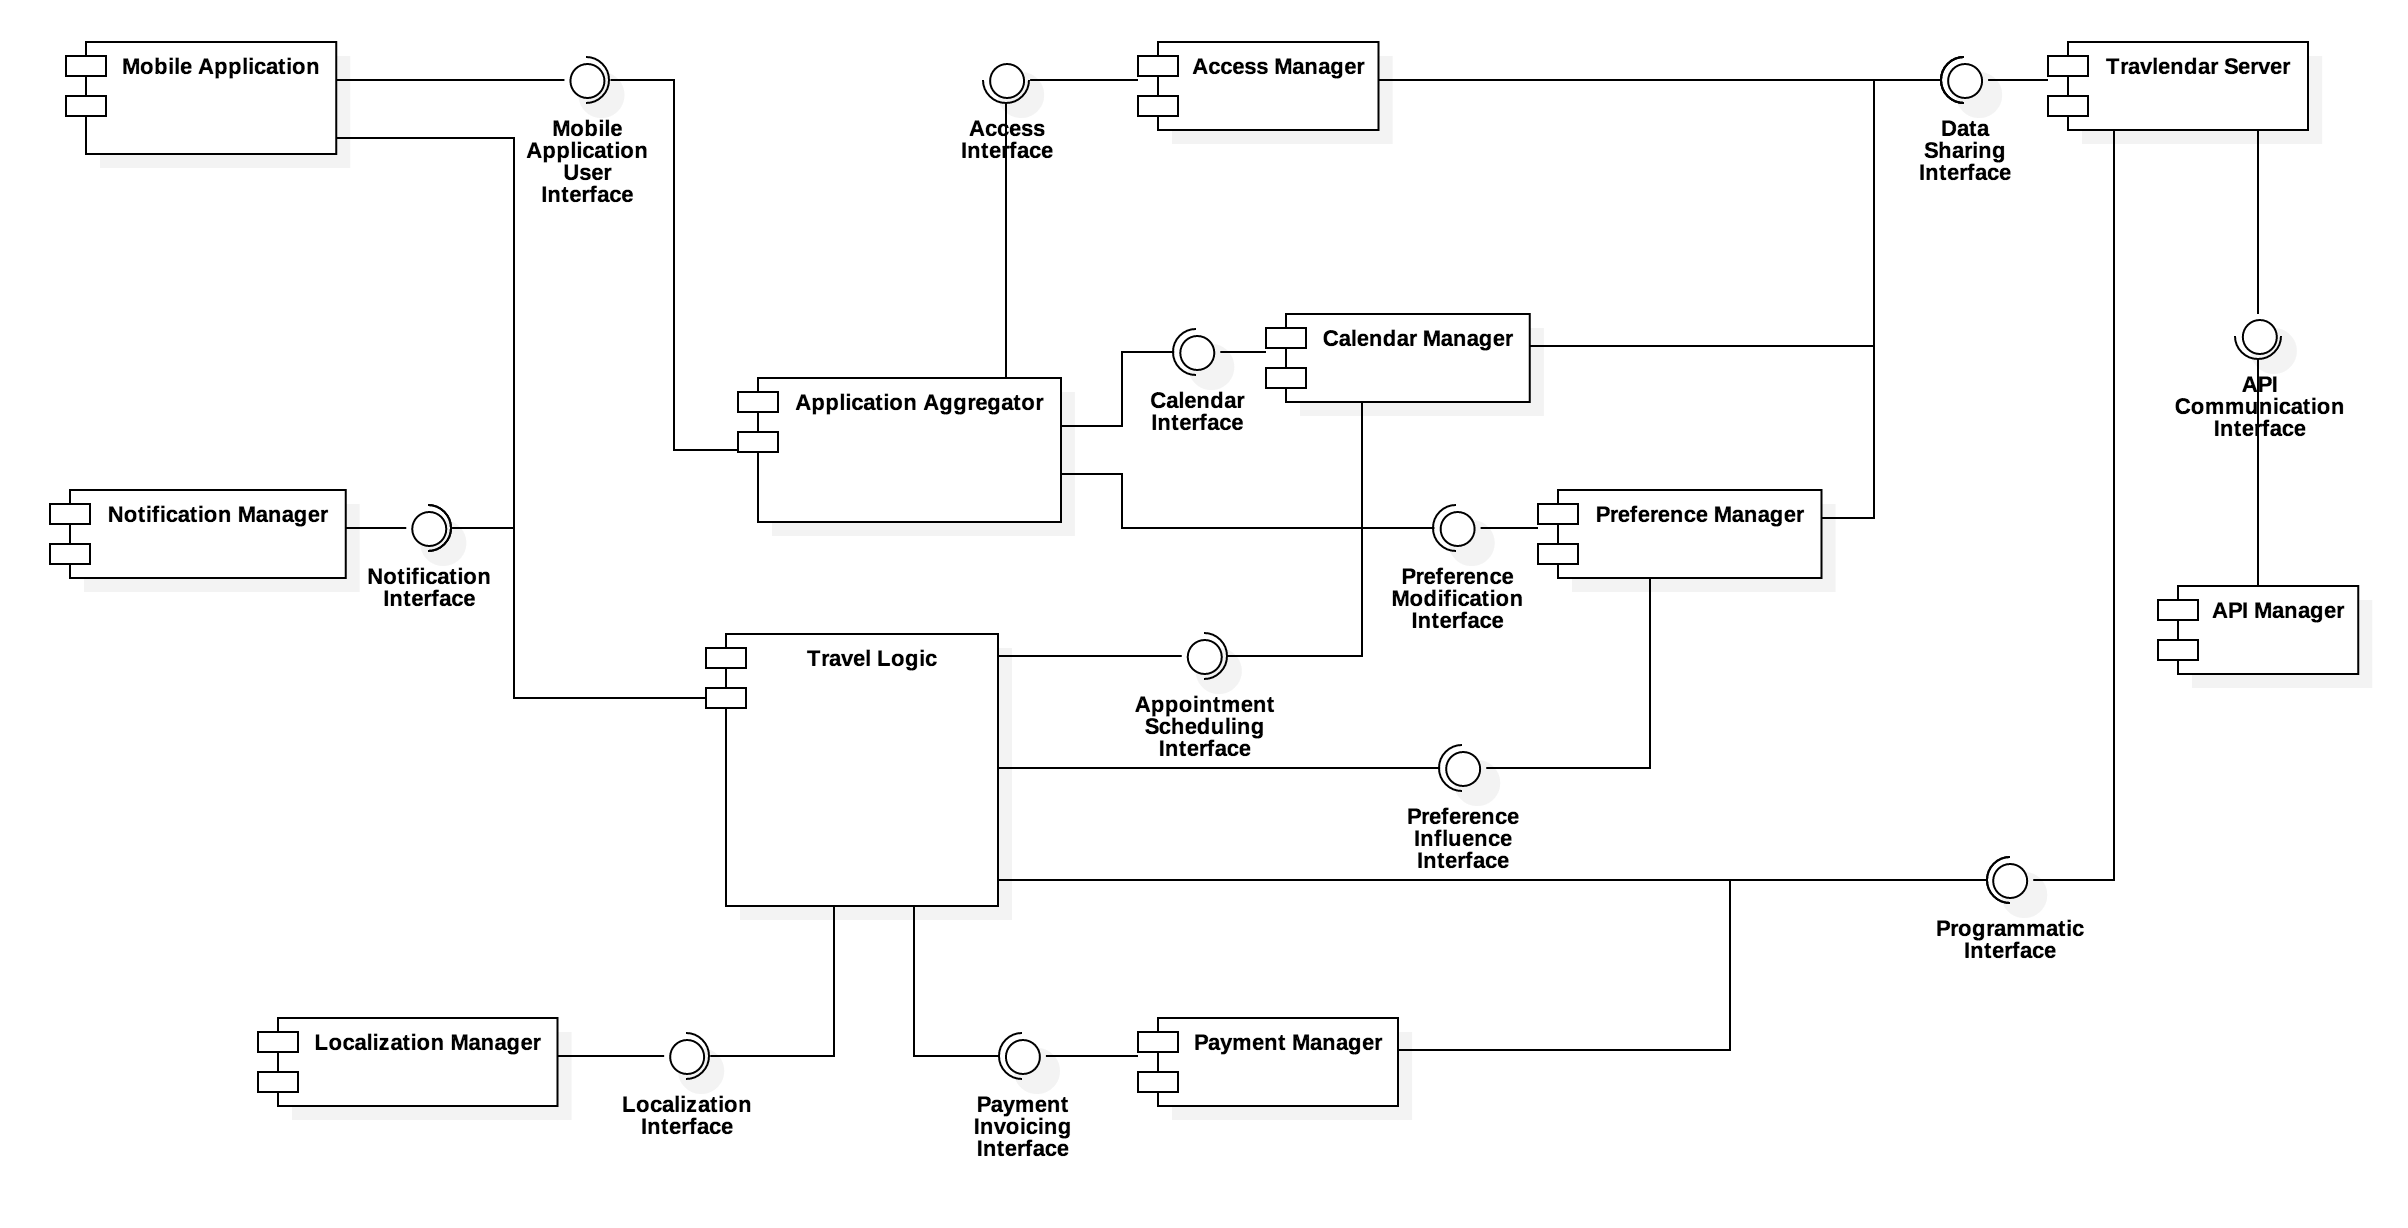
\includegraphics[width = \textwidth]{UML/componentDiagrams/highLevel}
		\caption{High level view}
		\label{componentHighLevel}
	\end{figure}

\paragraph{Mobile Application}
	This component represents the view of the User over its system. It’s split in two sub-components, Guest-view and User-view, which represents the two different ways an human interaction can be instaurated with the system.

	\begin{figure}[H]
		\centering
		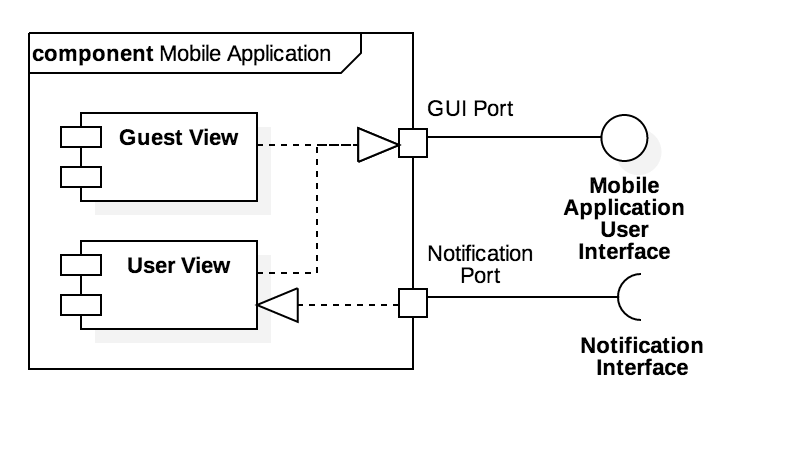
\includegraphics[scale = 0.2]{UML/componentDiagrams/mobileApplication}
	\end{figure}


\paragraph{Application Aggregator}
	This component works, unsuprisingly, as a collector of the different information \textit{Travlendar+} manages. It allows an easy management of every piece of information and allows us to avoid an high number of interfaces among the different components. 'Profile Manager' specifies the profile setting of the current user, while 'User Action Handler' allows us to register User's input.
	
	\begin{figure}[H]
		\centering
		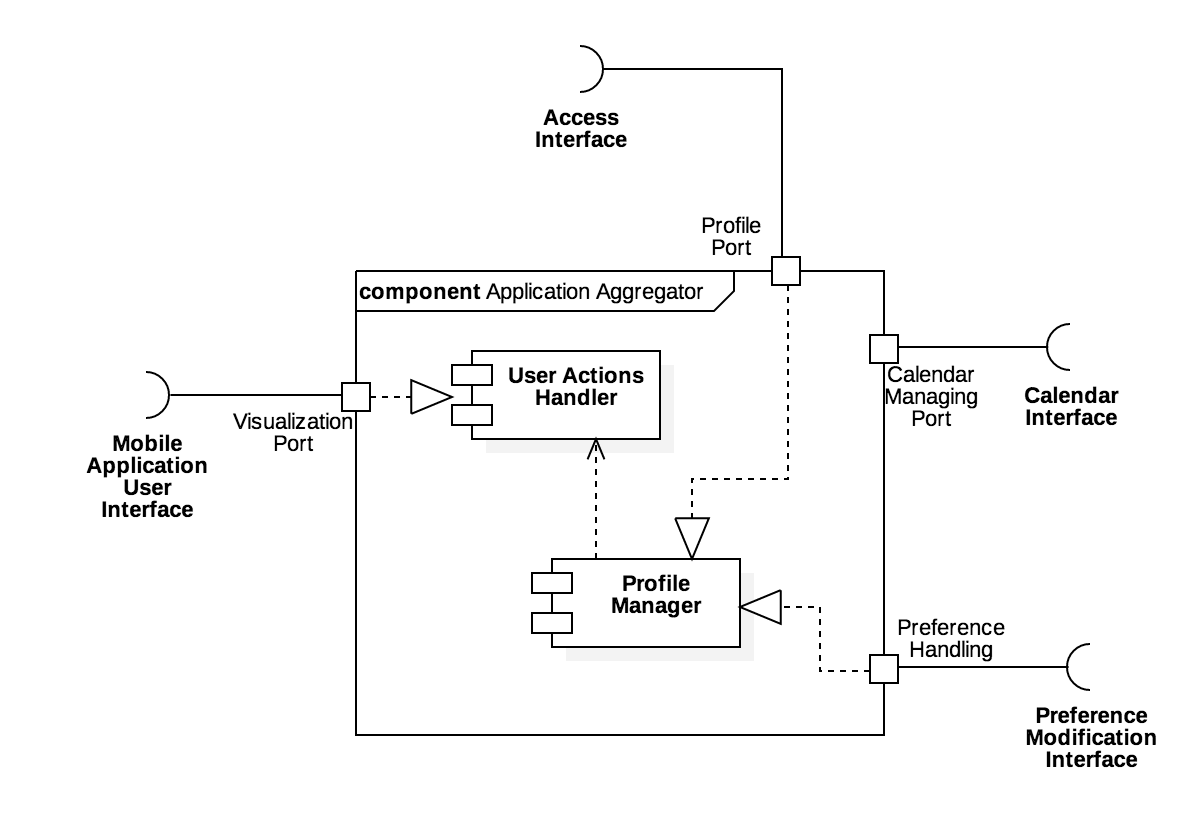
\includegraphics[scale = 0.2]{UML/componentDiagrams/applicationAggregator}
	\end{figure}
 
\paragraph{Calendar Manager}
	This component is divided into 'Appointments' and 'Breaks' sub-components, which track the appointments inserted by the User together with his breaks, and 'Trips', which is the list of trips arranged by the scheduler for every appointment. The sub-component 'Appointment Aggregator' serves the purpose of listing and presenting the content of the other two sub-components.
	
	\begin{figure}[H]
		\centering
		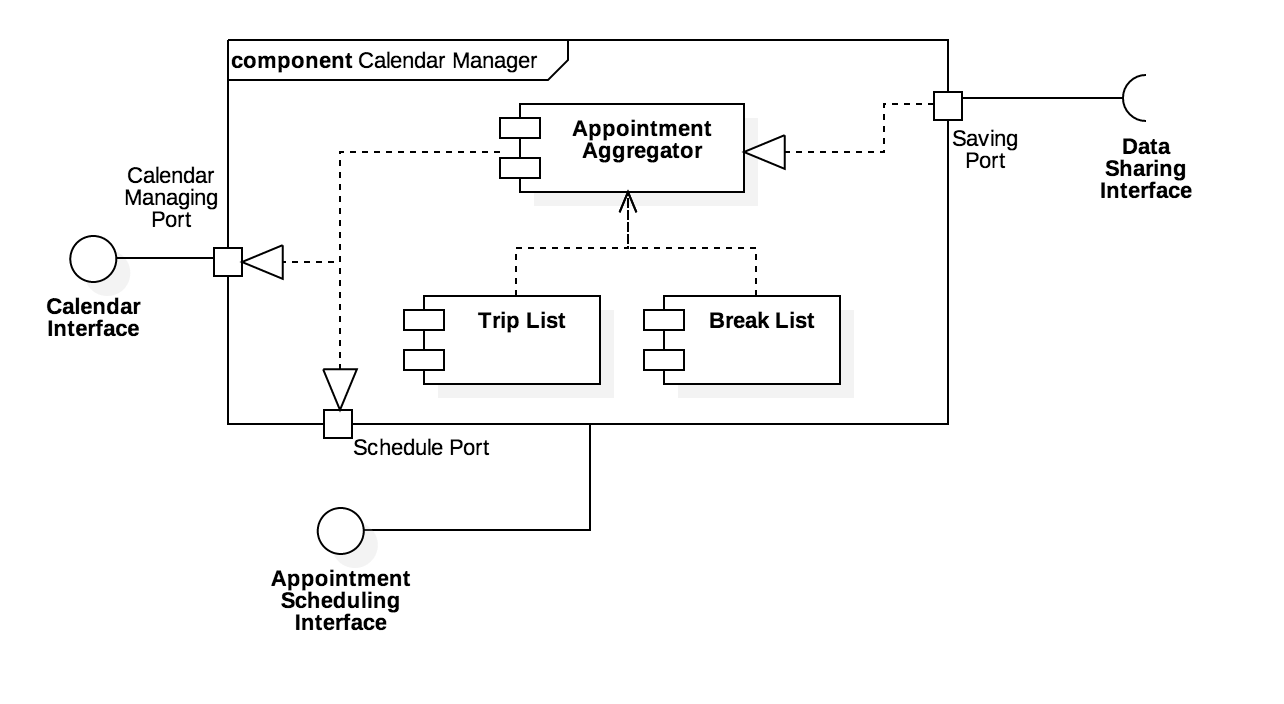
\includegraphics[scale = 0.2]{UML/componentDiagrams/calendarManager}
	\end{figure}
 

\paragraph{Preference Manager}
	This component serves the purpose of keeping track of the preferences expressed by the User. 'Season Pass Handler' takes care of storing season passes; 'Excluded Vehicles List' cuts off from the scheduler results involving a selection of banned transportation means, 'Preferences List' covers the remaining and wider spectrum of User's choices. 'Preference Handler' is the sub-component that manages the other ones and that communicates outside Preference Manager.

	\begin{figure}[H]
		\centering
		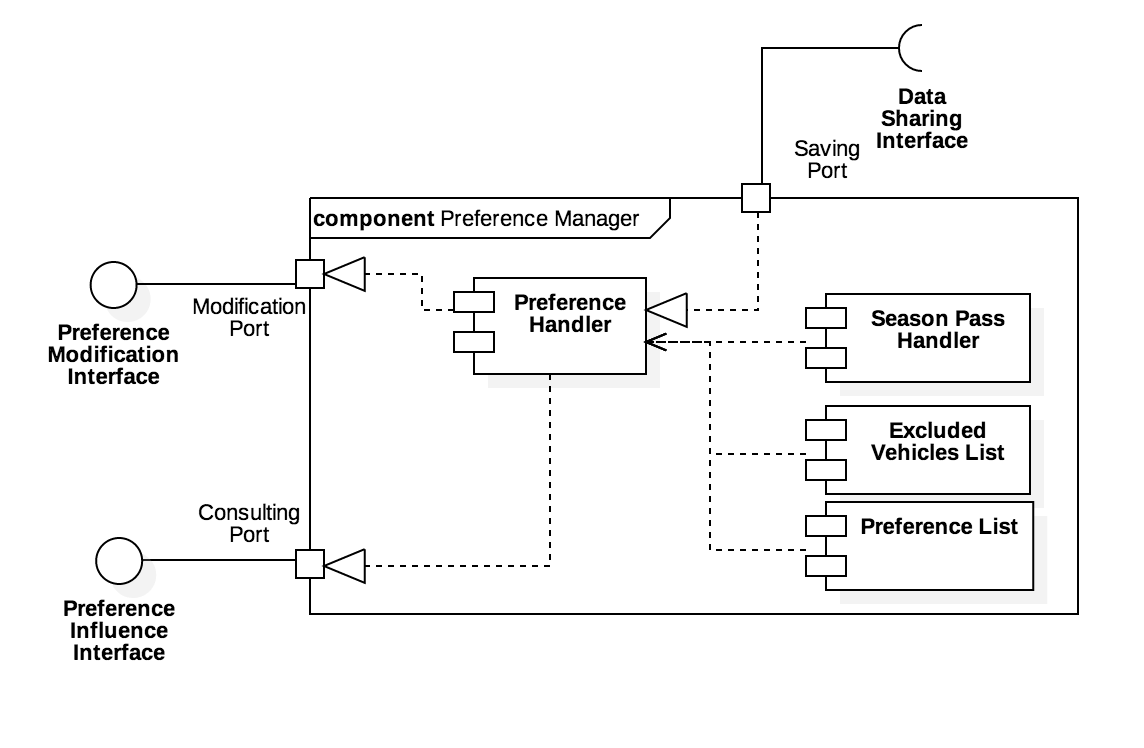
\includegraphics[scale = 0.2]{UML/componentDiagrams/preferenceManager}
	\end{figure}
	

\paragraph{Travlendar Server} 
	This component represents the \textit{Travlendar Server} whose purpose is to store User's preferences, access data and personal information. It is modeled by its 'DBMS' component, which stores Timetables and Preferences and the 'API Request Dispatcher', which forwards requests to external agents.

	\begin{figure}[H]
		\centering
		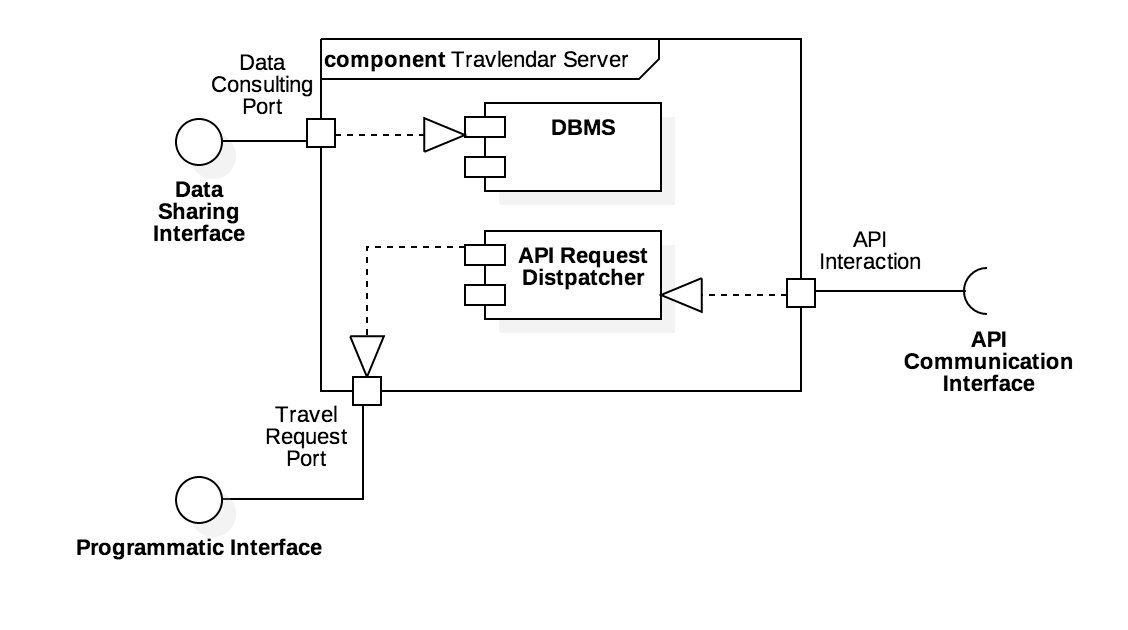
\includegraphics[scale = 0.2]{UML/componentDiagrams/travlendarServer}
	\end{figure}
	

\paragraph{Travel Logic Manager}
	This component is split into two sub-components: 'Scheduler' is the fundamental block that aims at scheduling and arranging User appointments and breaks via the the corresponding trips, 'DistanceManager' is the block whose purpose is to organize and present travel times to the scheduler in order to have them sorted out and well-managed.

	\begin{figure}[H]
		\centering
		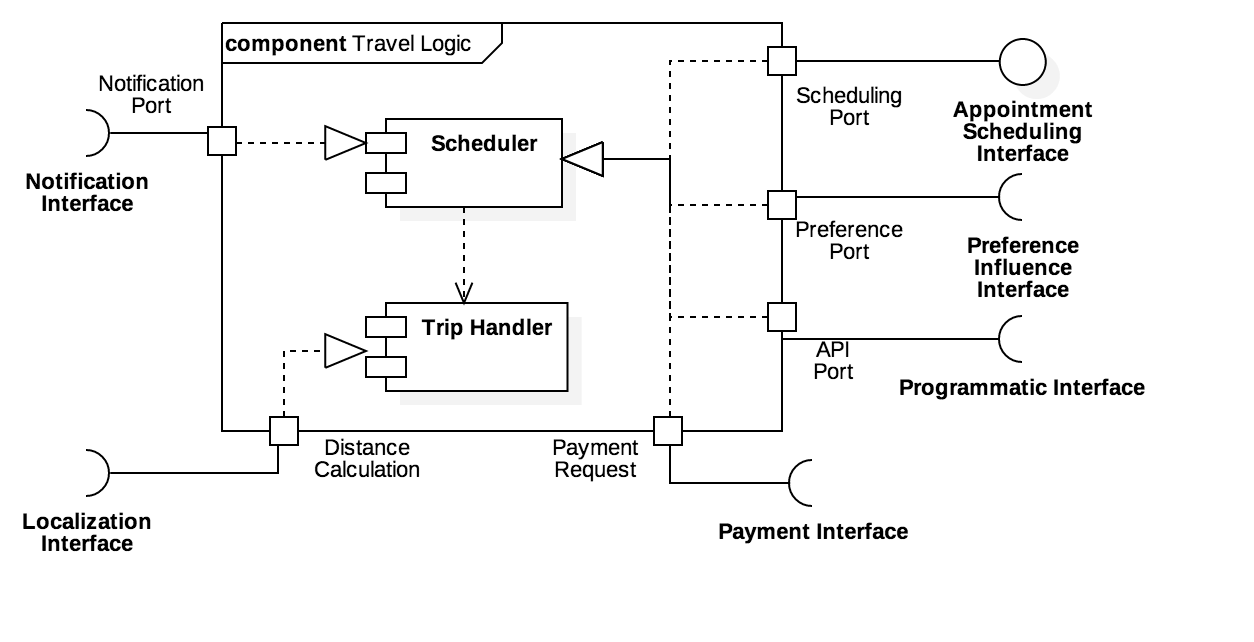
\includegraphics[scale = 0.2]{UML/componentDiagrams/travelLogic}
	\end{figure}
	

\paragraph{Payment Manager}
	This component deals with the recording of purchases and their associated credit cards.
	The sub-component 'Payment Handler' tracks purchase records and interacts with the required apps installed on the mobile device, while 'Purchase History' is an exploitable and rational organizations of the credit cards used by the user.

	\begin{figure}[H]
		\centering
		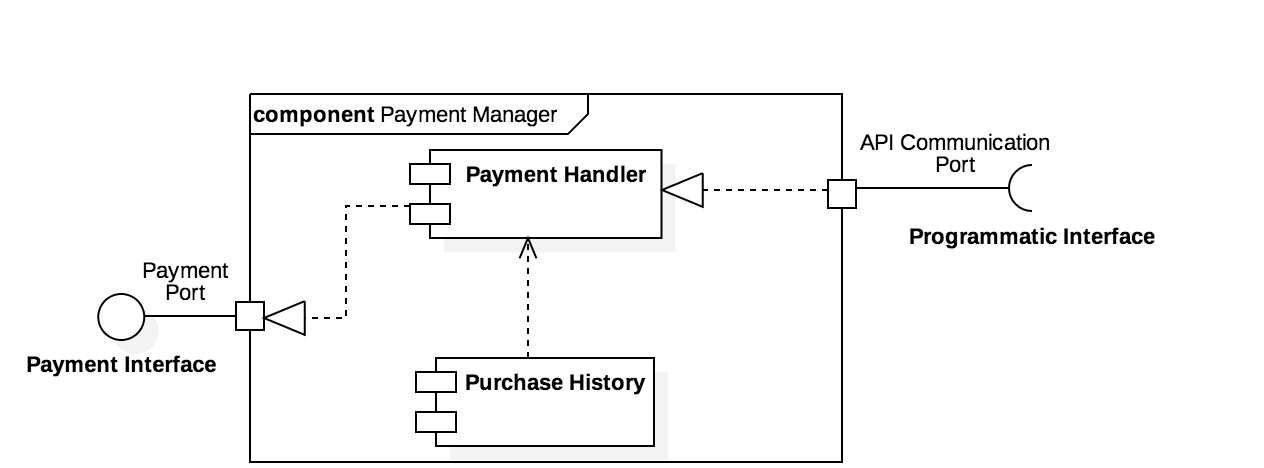
\includegraphics[scale = 0.2]{UML/componentDiagrams/paymentManager}
	\end{figure}
	

\paragraph{API Manager} 
	This component is critical in order to provide a functioning Travel Logic: it gathers the interactions with all external APIs.
	Here are listed the APIs the mobile application project starts with : Google Maps API, Google Transit API, Open Weather Map API, Car2Go and BikeMi API.
	The last couple is for reference only, as already pointed in the RASD. Naturally, the list of external services can be expanded.
	The 'Listener' component serves the purpose of forwarding requests and receives the desired inputs.
	
	\begin{figure}[H]
		\centering
		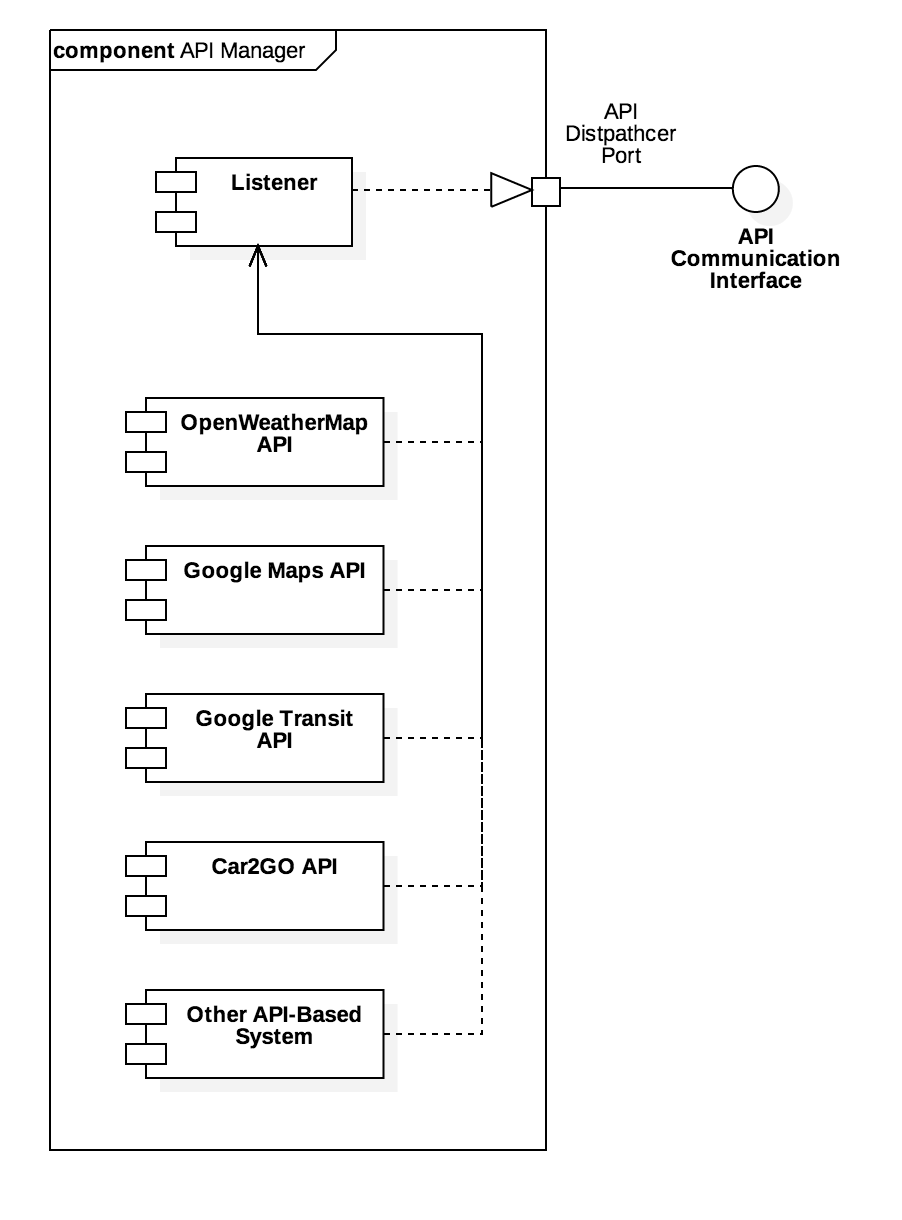
\includegraphics[scale = 0.2]{UML/componentDiagrams/APIManager}
	\end{figure}
	
	
\paragraph{Notification Manager}
	This component allows the notification system to warn users in the cases events partially or completely overlap according to the scheduler.

\paragraph{Localization Manager}
	This component represents the localization functionalities of the mobile application.
	
\begin{landscape}
	\begin{figure}
		\centering
		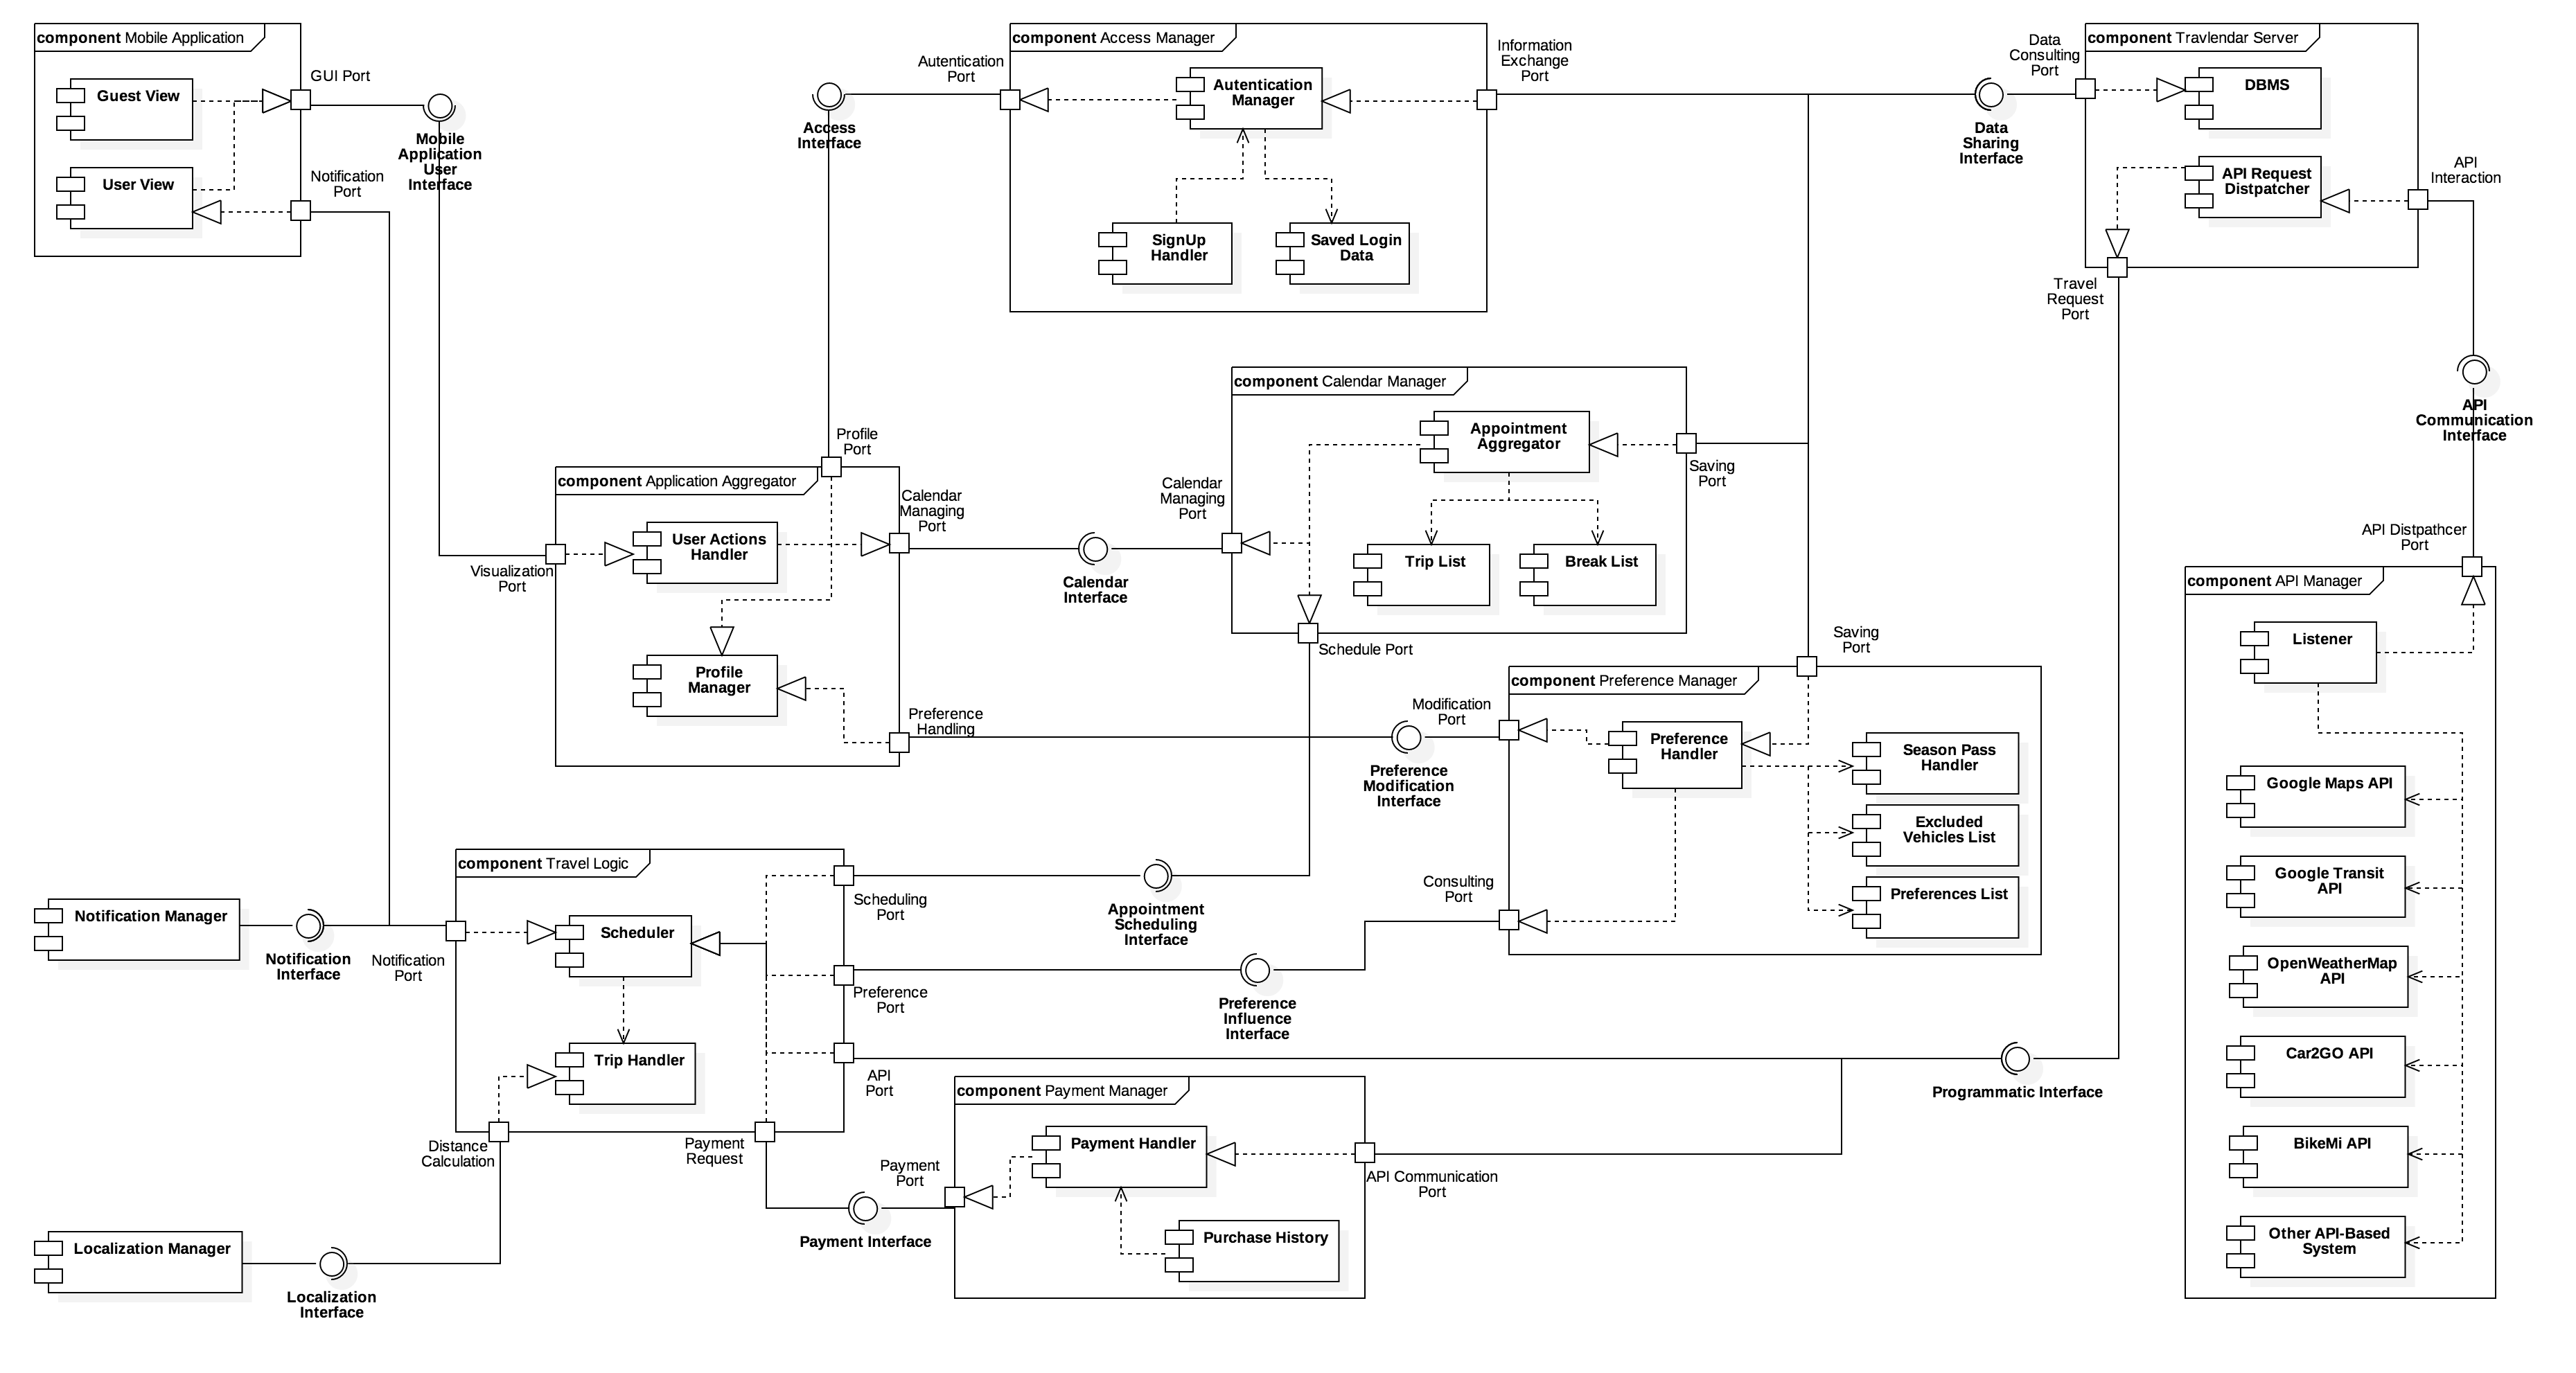
\includegraphics[height= 0.9\textheight]{UML/componentDiagrams/detailedLevel}
		\caption{Detailed level view}
		\label{detailedHighLevel}
	\end{figure}
\end{landscape}





	
\subsection{Deployment View}
	%The Component Diagram shown below describes the logical components of the system we are to develop, from a very high-level description on to a more detailed one. This diagram does not take into account the deployment phase, hence it doesn’t describe the logical layer of the system in terms of the physical tiers where it is deployed.

\begin{figure}[H]
		\centering
		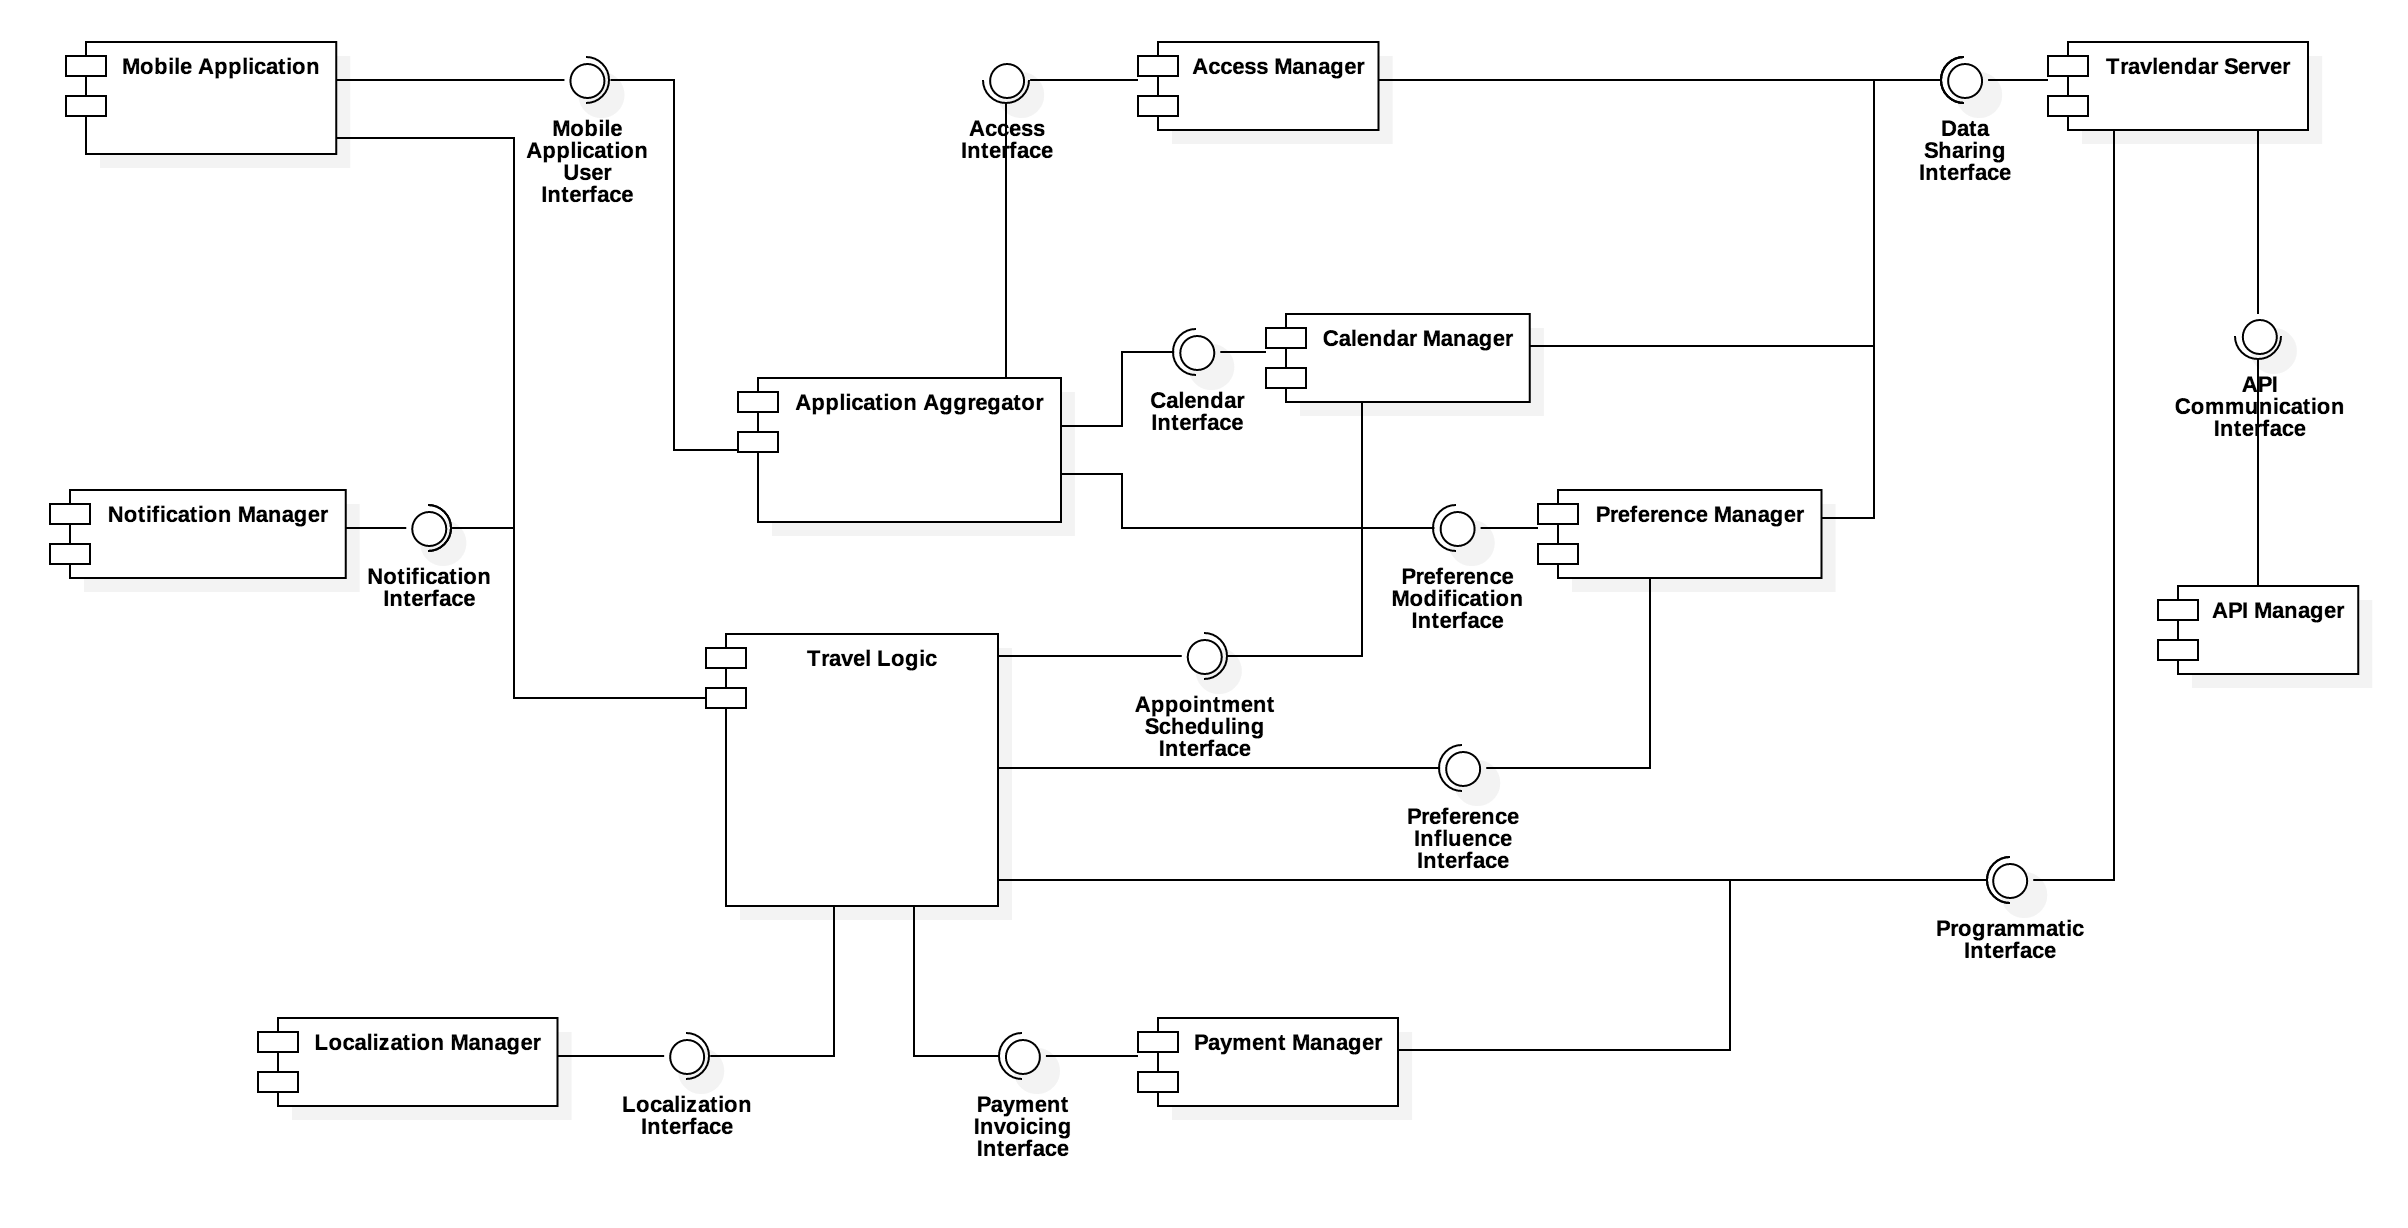
\includegraphics[width = \textwidth]{UML/componentDiagrams/highLevel}
		\caption{High level view}
		\label{componentHighLevel}
	\end{figure}

\paragraph{Mobile Application}
	This component represents the view of the User over its system. It’s split in two sub-components, Guest-view and User-view, which represents the two different ways an human interaction can be instaurated with the system.

	\begin{figure}[H]
		\centering
		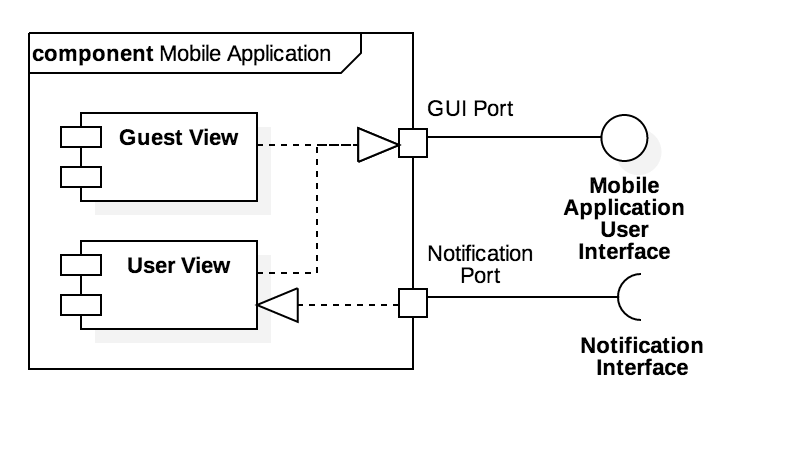
\includegraphics[scale = 0.2]{UML/componentDiagrams/mobileApplication}
	\end{figure}


\paragraph{Application Aggregator}
	This component works, unsuprisingly, as a collector of the different information \textit{Travlendar+} manages. It allows an easy management of every piece of information and allows us to avoid an high number of interfaces among the different components. 'Profile Manager' specifies the profile setting of the current user, while 'User Action Handler' allows us to register User's input.
	
	\begin{figure}[H]
		\centering
		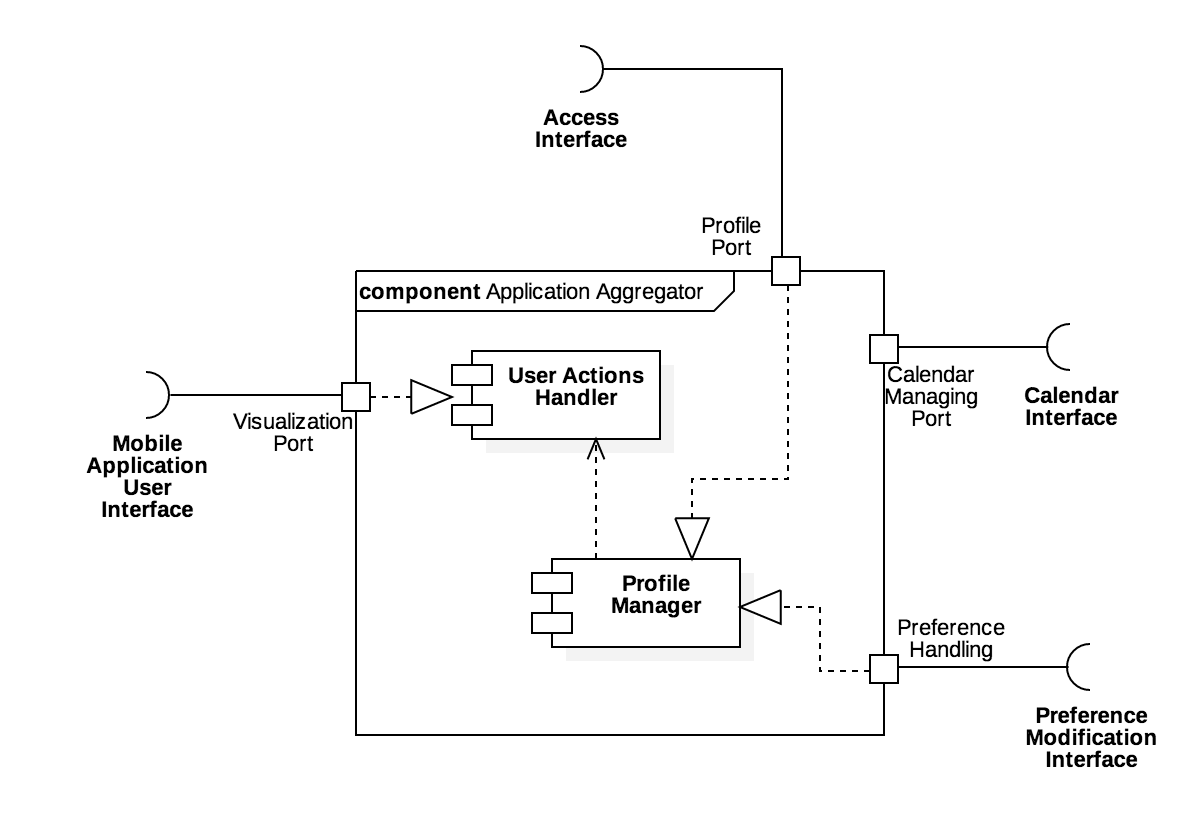
\includegraphics[scale = 0.2]{UML/componentDiagrams/applicationAggregator}
	\end{figure}
 
\paragraph{Calendar Manager}
	This component is divided into 'Appointments' and 'Breaks' sub-components, which track the appointments inserted by the User together with his breaks, and 'Trips', which is the list of trips arranged by the scheduler for every appointment. The sub-component 'Appointment Aggregator' serves the purpose of listing and presenting the content of the other two sub-components.
	
	\begin{figure}[H]
		\centering
		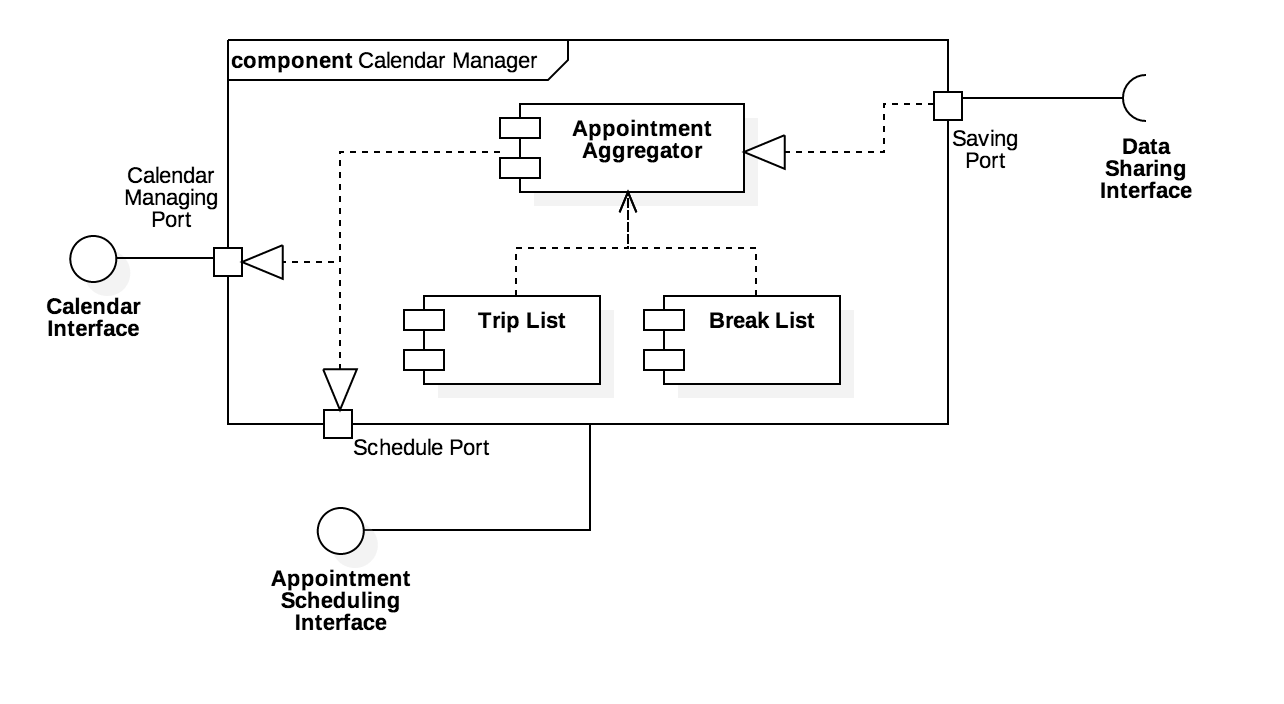
\includegraphics[scale = 0.2]{UML/componentDiagrams/calendarManager}
	\end{figure}
 

\paragraph{Preference Manager}
	This component serves the purpose of keeping track of the preferences expressed by the User. 'Season Pass Handler' takes care of storing season passes; 'Excluded Vehicles List' cuts off from the scheduler results involving a selection of banned transportation means, 'Preferences List' covers the remaining and wider spectrum of User's choices. 'Preference Handler' is the sub-component that manages the other ones and that communicates outside Preference Manager.

	\begin{figure}[H]
		\centering
		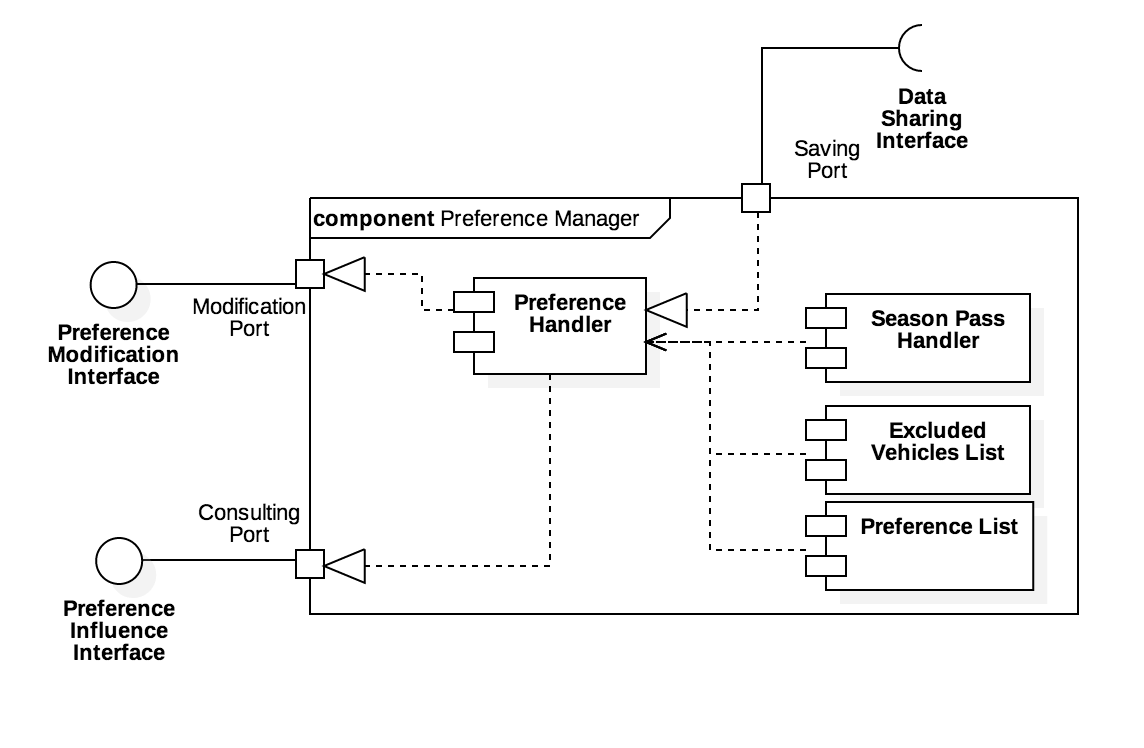
\includegraphics[scale = 0.2]{UML/componentDiagrams/preferenceManager}
	\end{figure}
	

\paragraph{Travlendar Server} 
	This component represents the \textit{Travlendar Server} whose purpose is to store User's preferences, access data and personal information. It is modeled by its 'DBMS' component, which stores Timetables and Preferences and the 'API Request Dispatcher', which forwards requests to external agents.

	\begin{figure}[H]
		\centering
		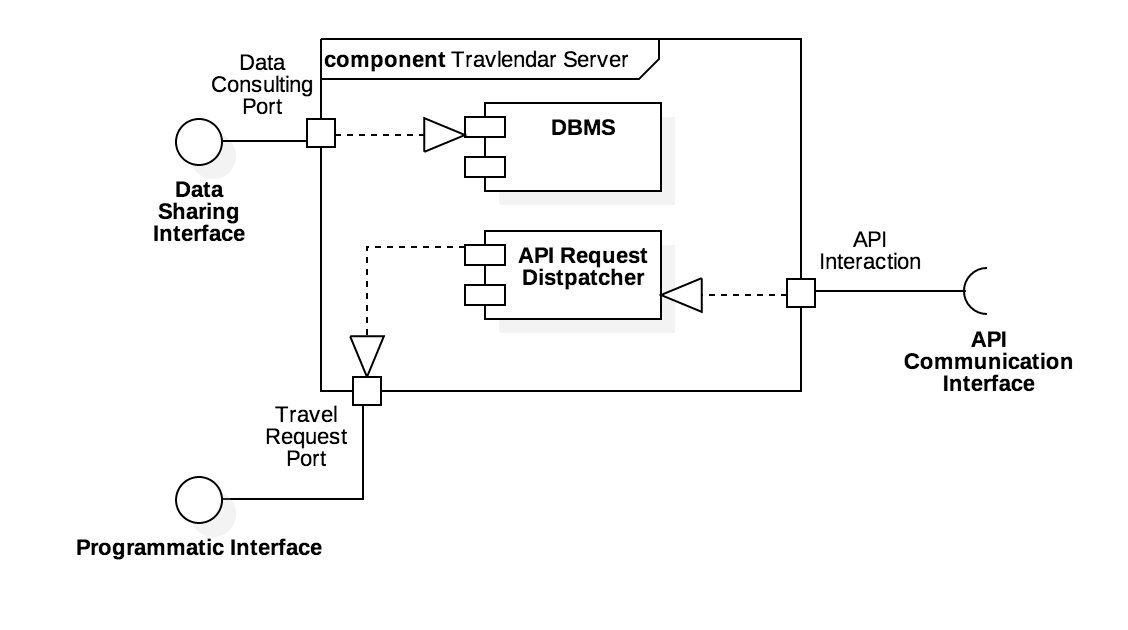
\includegraphics[scale = 0.2]{UML/componentDiagrams/travlendarServer}
	\end{figure}
	

\paragraph{Travel Logic Manager}
	This component is split into two sub-components: 'Scheduler' is the fundamental block that aims at scheduling and arranging User appointments and breaks via the the corresponding trips, 'DistanceManager' is the block whose purpose is to organize and present travel times to the scheduler in order to have them sorted out and well-managed.

	\begin{figure}[H]
		\centering
		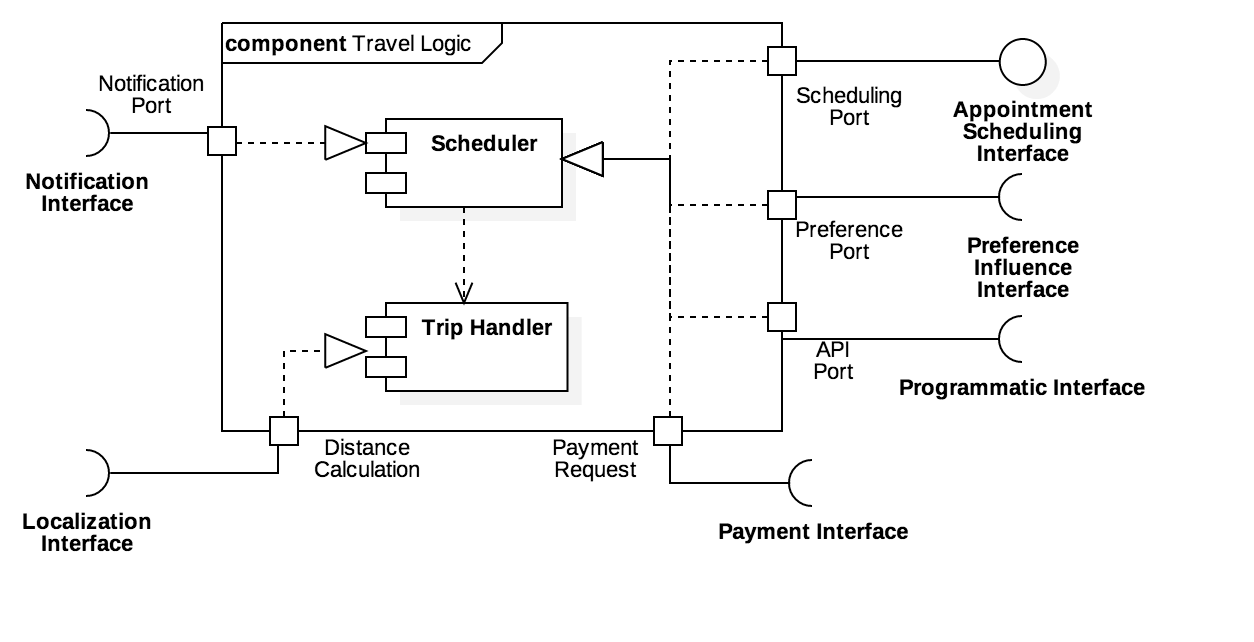
\includegraphics[scale = 0.2]{UML/componentDiagrams/travelLogic}
	\end{figure}
	

\paragraph{Payment Manager}
	This component deals with the recording of purchases and their associated credit cards.
	The sub-component 'Payment Handler' tracks purchase records and interacts with the required apps installed on the mobile device, while 'Purchase History' is an exploitable and rational organizations of the credit cards used by the user.

	\begin{figure}[H]
		\centering
		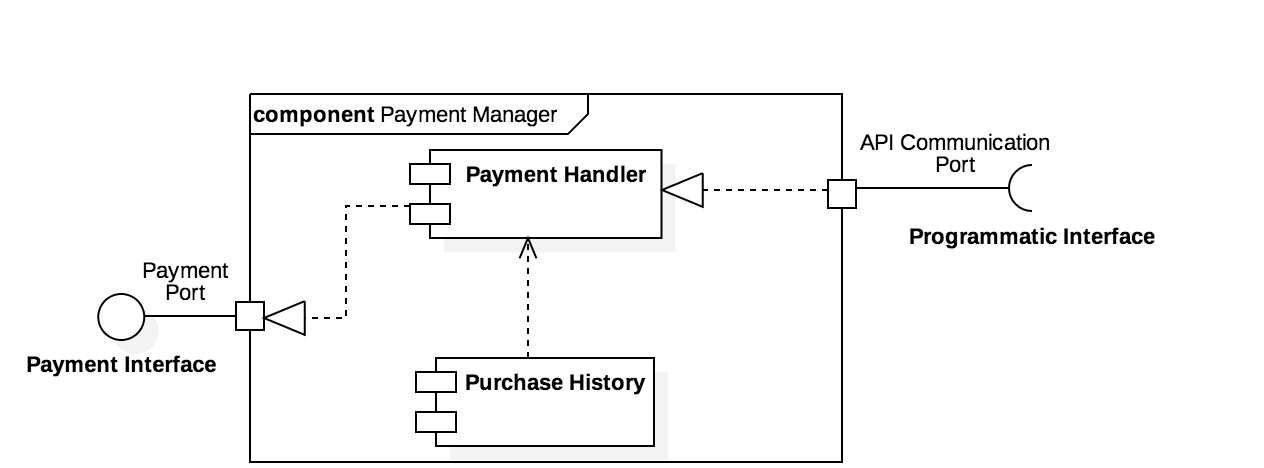
\includegraphics[scale = 0.2]{UML/componentDiagrams/paymentManager}
	\end{figure}
	

\paragraph{API Manager} 
	This component is critical in order to provide a functioning Travel Logic: it gathers the interactions with all external APIs.
	Here are listed the APIs the mobile application project starts with : Google Maps API, Google Transit API, Open Weather Map API, Car2Go and BikeMi API.
	The last couple is for reference only, as already pointed in the RASD. Naturally, the list of external services can be expanded.
	The 'Listener' component serves the purpose of forwarding requests and receives the desired inputs.
	
	\begin{figure}[H]
		\centering
		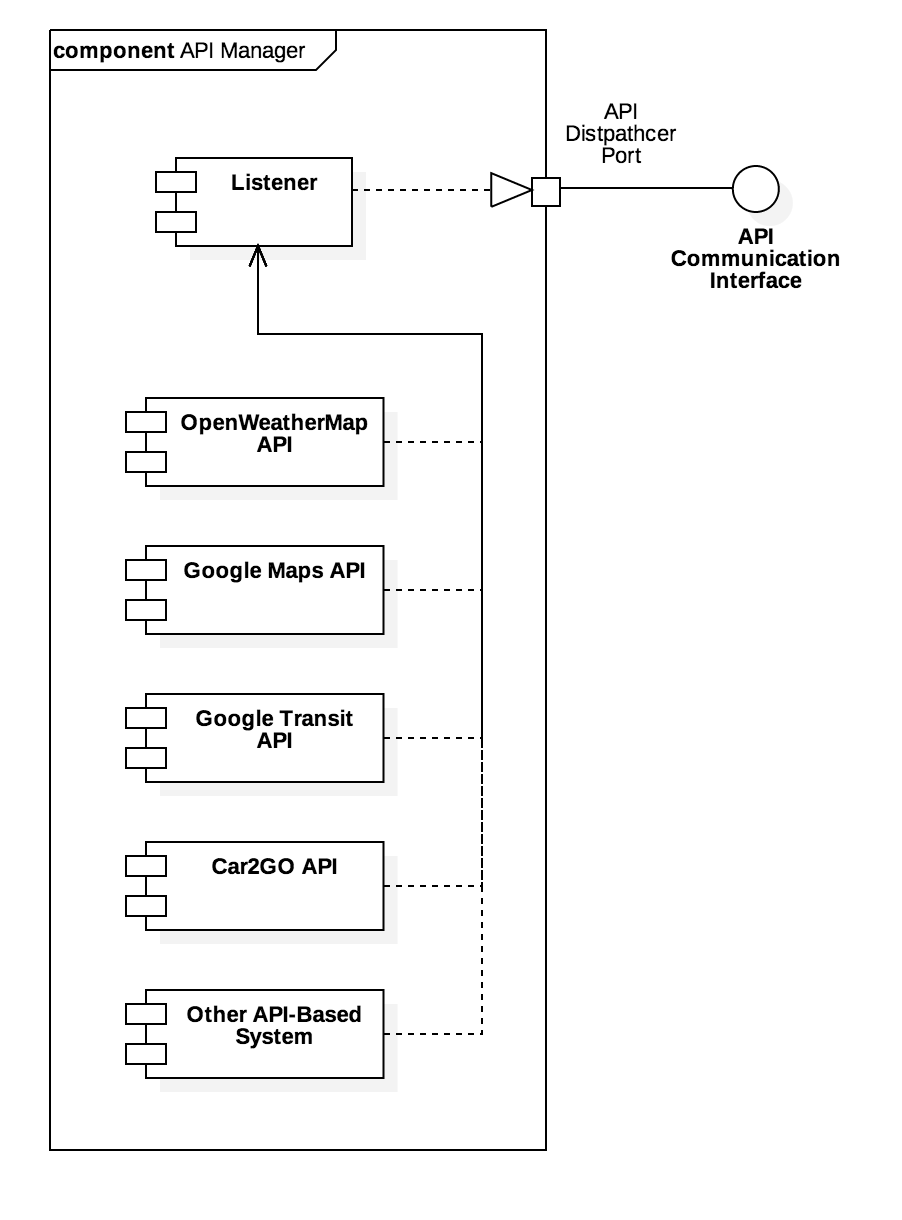
\includegraphics[scale = 0.2]{UML/componentDiagrams/APIManager}
	\end{figure}
	
	
\paragraph{Notification Manager}
	This component allows the notification system to warn users in the cases events partially or completely overlap according to the scheduler.

\paragraph{Localization Manager}
	This component represents the localization functionalities of the mobile application.
	
\begin{landscape}
	\begin{figure}
		\centering
		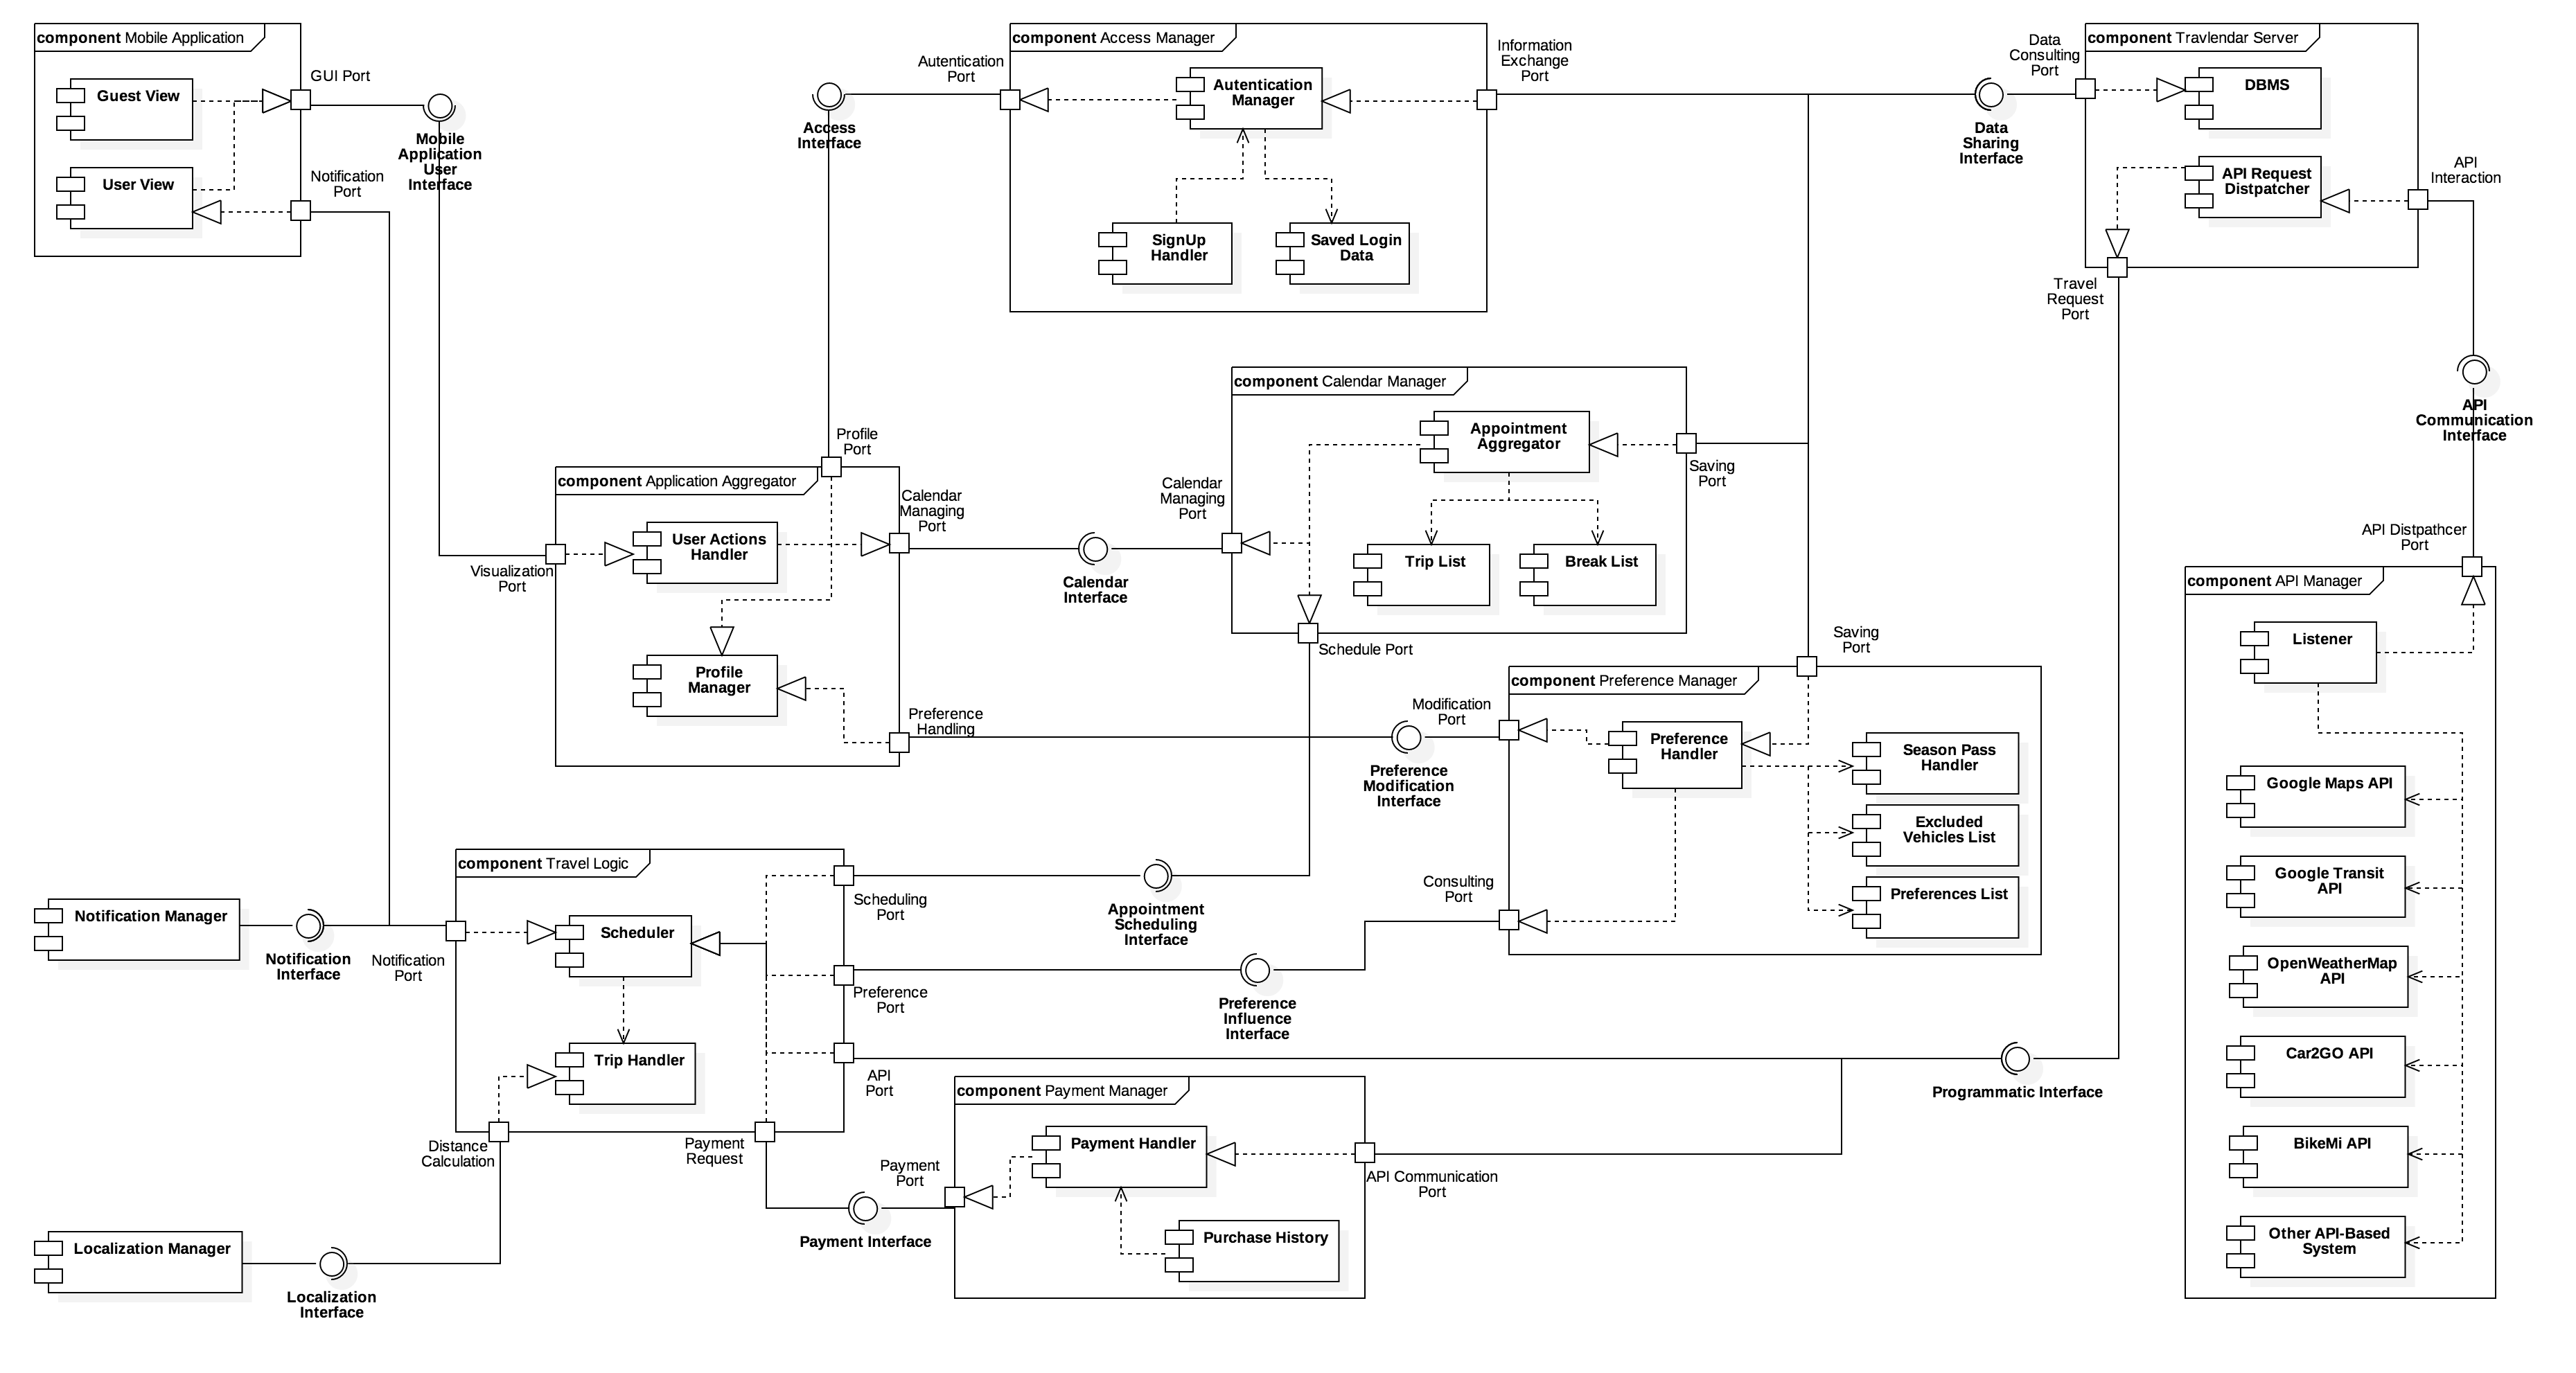
\includegraphics[height= 0.9\textheight]{UML/componentDiagrams/detailedLevel}
		\caption{Detailed level view}
		\label{detailedHighLevel}
	\end{figure}
\end{landscape}





	
\subsection{Runtime view}
	%\input{subsections/section2/rutimeView.tex}

\subsection{Component Interfaces}
	%In this section we will show the component Interfaces. For each one are reported the main functionalities.
Nevertheless we need to keep in mind that in further implementations these functions can be splitted into less complex ones.

\begin{figure}[H]

	\begin{subfigure}[t]{0.3\linewidth}
		\centering
		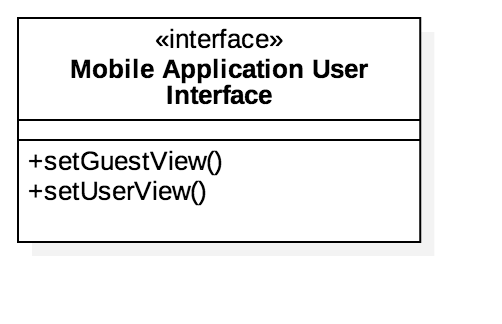
\includegraphics[width=\linewidth]{UML/Interfaces/mobileApplicationUserInterface}
		\caption{Mobile Application User Interface}
	\end{subfigure}
	~
	\begin{subfigure}[t]{0.3\linewidth}
		\centering
		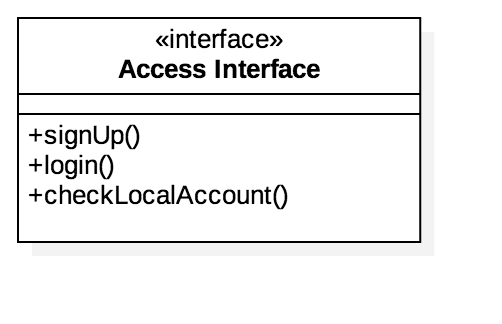
\includegraphics[width=\linewidth]{UML/Interfaces/accessInterface}
		\caption{Access Interface}
	\end{subfigure}
	~	
	\begin{subfigure}[t]{0.3\linewidth}
		\centering
		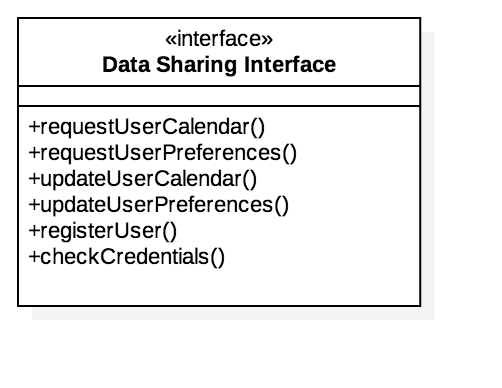
\includegraphics[width=\linewidth]{UML/Interfaces/dataSharingInterface}
		\caption{Daba Sharing Interface}
	\end{subfigure}
	\hfill
	\vskip0.75cm
	
	
	\begin{subfigure}[t]{0.3\linewidth}
		\centering
		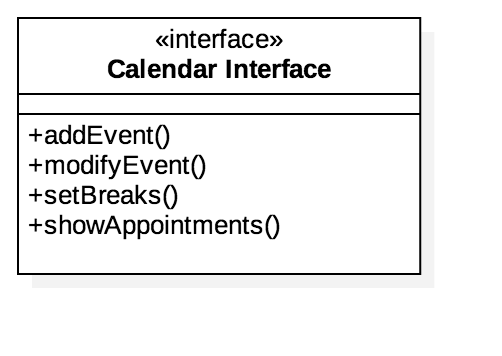
\includegraphics[width=\linewidth]{UML/Interfaces/calendarInterface}
		\caption{Calendar Interface}
	\end{subfigure}
	~
	\begin{subfigure}[t]{0.3\linewidth}
		\centering
		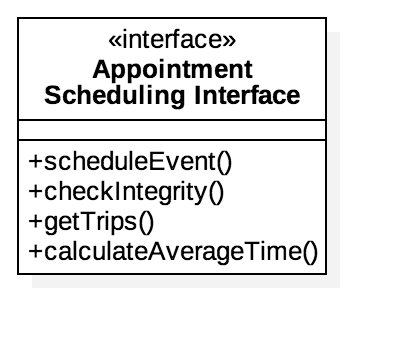
\includegraphics[width=\linewidth]{UML/Interfaces/appointmentSchedulingInterface}
		\caption{Appointment Scheduling Interface}
	\end{subfigure}
	~
	\begin{subfigure}[t]{0.3\linewidth}
		\centering
		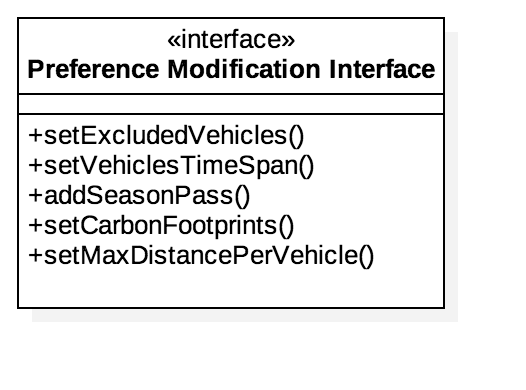
\includegraphics[width=\linewidth]{UML/Interfaces/preferenceModificationInterface}
	\caption{Preference Modification Interface}
	\end{subfigure}
	\hfill
	\vskip0.75cm
	
	
	\begin{subfigure}[t]{0.3\linewidth}
		\centering
		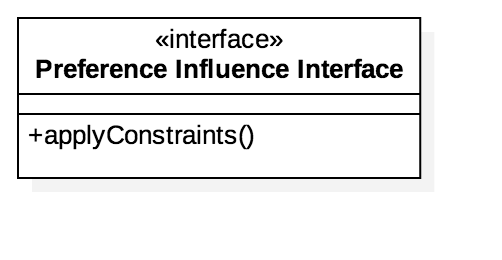
\includegraphics[width=\linewidth]{UML/Interfaces/preferenceInfluenceInterface}
		\caption{Preference Influence Interface}
	\end{subfigure}
	~
	\begin{subfigure}[t]{0.3\linewidth}
		\centering
		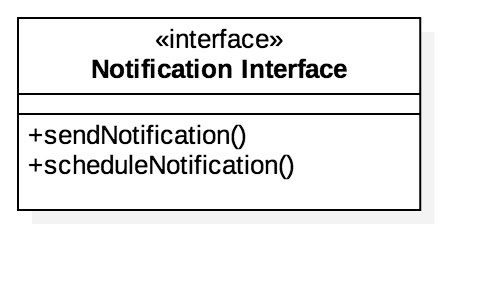
\includegraphics[width=\linewidth]{UML/Interfaces/notificationInterface}
		\caption{Notification Interface}
	\end{subfigure}
	~
	\begin{subfigure}[t]{0.3\linewidth}
		\centering
		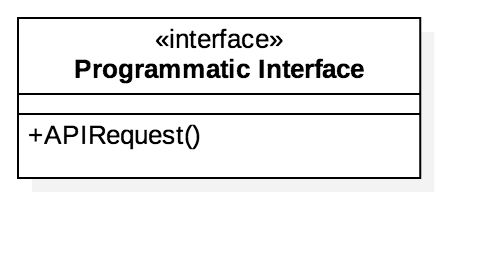
\includegraphics[width=\linewidth]{UML/Interfaces/programmaticInterface}
		\caption{Programmatic Interface}
	\end{subfigure}
\end{figure}	


\begin{figure}[H]\ContinuedFloat
	\begin{subfigure}[t]{0.3\linewidth}
		\centering
		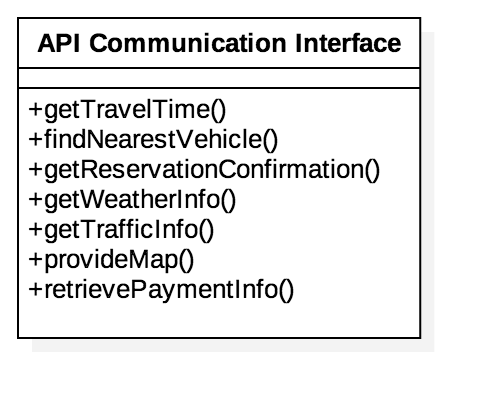
\includegraphics[width=\linewidth]{UML/Interfaces/APICommunicationInterface}
		\caption{API Communication Interface}
	\end{subfigure}
	~
	\begin{subfigure}[t]{0.3\linewidth}
		\centering
		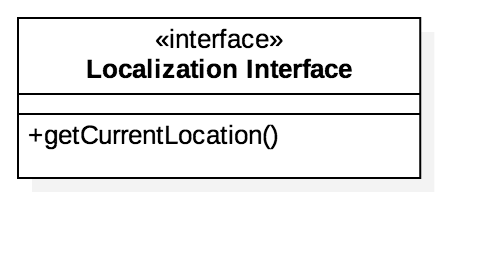
\includegraphics[width=\linewidth]{UML/Interfaces/localizationInterface}
		\caption{Localization Interface}
	\end{subfigure}
	~
	\begin{subfigure}[t]{0.3\linewidth}
		\centering
		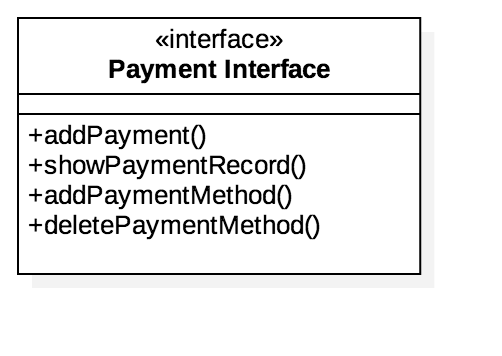
\includegraphics[width=\linewidth]{UML/Interfaces/paymentInterface}
		\caption{Payment Interface}
	\end{subfigure}
	
	\caption{List of Interfaces}
\end{figure}

\subsection{Architectural Styles}
	
[Architectural Style]

For our system architecture we adopt a 3-tier client/server architecture : we'll have a Mobile Application Clients, a Travlendar
 Server and a Data Storage Layer.


Mobile Application Clients : This layer is represented by the Travlendar+ Application, a thick client and an interactive and dinamic GUI.
The application will be written in Java for increased portability and will be able both to geo-localize its user and to communciate with the core of the travel : this is the foundation of information synching and requests forwarding to APIs.

Travlendar+ Server : The business Server runs the business logic. Its main duty is to forward requests of the users to the Data layer and external APIs while saving all necessary users' preferences and timetables. These operations are executed under a microservice architectural pattern.

The Data Layer : This layer comprehends both the DBMS which stores and manages users' preferences and timetables and the external service agents (objects which call external services). In the former case it is required the capability of providing data through SQL queries using ODBC protocol, while in the latter it is required a good implementation of the ad-hoc functions of the external APIs.
(link Microsoft)

Patterns

Pattern are mostly required to smooth the construction of our system. In particular, we'll be using a MVC (Model - View - Control) Pattern for our mobile application, Adapter (??), Client/Server and Single Instance component.

MVC is used to define our Java mobile application : the view will be the dynamic GUI, the Travel Logic the control and the model will be the data received from the APIs and the locally stored timetables and trips.


Single Instance component will be mostly useful when treating the components of the mobile application : components like Access Manager or Travel Logic will be the ones mainly touched by this pattern.

Client/Server pattern is the one we adopted to shape the interactions between our mobile application (the client) and the Travlendar+ Server (i.e, the server). Reasons for adoption have mainly been the simplicity and widespread use of the model.


%Vecchia parte di Michele!
In particolare ci serviremo del pattern MVC (Model View Control) molto utile perchè ci permette di separare la logica Business dalla logica di Presentazione. In questo caso il Database interpreterà il ruolo del Model, Mobile Application interpreterà il ruolo di View, e il Server sarà il Control. 

		
%%% 3 -ALGORITHM DESIGN  %%%
	\newpage
	\section{Algorithm Design}
		% RANK SOLUTIONS %
\paragraph{solution Ranking}
This algorithm shows how System ranks all the feasible solution based provided by the external sources, like Public Transportation, via Car, Bike or Foot, depending on:
	\begin{itemize}
		\item[•] time needed for completing the trip.
		\item[•] number of subtrips (only for Public Tranportation).
		\item[•] if the Car have to be used in other trips on that day.
		\item[•] money needed for the Tranportation Mean, calculated as:
			\begin{itemize}
				\item[-] public ticket cost for Public Services.
				\item[-] average fuel cost for Car.
				\item[-] tariff \euro /time for Sharing services.
			\end{itemize}
		\item[•] User preferences.
		\item[•] Weather forecast for the Appointment day (if and only if the Appointment is no longer than 15 days).
	\end{itemize}
	
	Since solutions have been already calculated individually, is supposed that every element in the input list has been already divided in subtrips either by the External API Manager or by Scheduler (see figure \ref{travelLogicDetail} and figure \ref{APIManagerDetail}) in a previous Step.
	Is also assumed that 'Public Service Manager' (see RASD Class Diagram) provides a list of different tranportation means, and all the consistent possible combinations of them.
	
	First of all Every element in the input list is filtered by the 'Excluded Vehicles List' (see figure \ref{preferenceManagerDetail})
	For remaining elements, every inner SubTrip time is compared with the average reference time that the User have to spend by going with owned Car or bike, or, if is a short distance, by going with foot, in order to categorize solutions in \textit{suitables}, \textit{valid alternatives}, and \textit{unconvenient}.
	
	
	
	Then for every category solutions:
	\begin{itemize}
		\item[-] items are orderd by \textit{time needed} and \textit{number of SubTrip}
		\item[-] if User has a Season Pass of a public transportation company, relative solutions are put on the highest rank.
		\item[-] solution cost are calculated, as aforementioned.
	\end{itemize}		
		
	If a solutions from lower category are advantageous with respect to 'higher' solutions, those are put again in the upper category.
	A solution is advantageous if \textit{time needed}s difference between the two category, defined as 
	\\ \quad $\Delta =  timeNeeded(bestUpperSolution) - timeNeeded(lowerSolution)$, \\
	is less than 15 minutes, and either is a cheaper solution or User has a Season Pass that doesn't belong to any other company of Upper-category solutions.
		
	If the Appointment is scheduled in less than 15 days, and weather forecast is predicted al \textit{non consistent for outdoor tripping}, solutions that expect a $total\_Outdoor\_Time$ defined as the sum of the time spent by walking and biking, greater than 3 minutes are downgraded in the respective category.

	If in the other Appointments of that day a proprietary Car solution is already scheduled, 'Only by Using Car' solution will be encouraged, but if and only if:

	In the end all the category \textit{suitables} and \textit{valid alternatives} are merged into an unique list made so that User can choose one.
	The algorithm return also the $bestSolution$ got by 'Poping' of the first element of the list, and the solution obtained by 'Only Walking' and 'Only by Using Car'.
	
	\vfill
	\begin{algorithm}[H]
\caption{Rank Solution}
	\KwData{Trip, List of Calculated Solutions, Preferences, Calendar}
	\KwResult{List of Ranked Solutions, Best Calculated Solution, Only Car Time, Only Walking Time}
		
	\bigskip
	\tcp{Calculate 'Only Car' and 'Only Walking' Solutions}
	$ carSolution \leftarrow \textbf{Scheduler}.carTime$\;
	$ bikeSolution \leftarrow \textbf{Scheduler}.walkingTime$\;
		
	\bigskip
	\tcp{Filtering Solutions based on $Preferences$}	
	\ForAll{Trip in Input\_List}{
		\If{Trip.AssignedTransportationMean() is in Excluded\_Vehicles\_List}{
			$ InputList.remove(Trip) $\;
		}
	}
	$ FilteredList \leftarrow InputList $\;

	\bigskip
	\tcp{Assign a category}	
	\ForAll{Trip in Filtered\_List}{
		$ \delta_{Advantage} \leftarrow 0$\;
		\ForEach{SubTrip in Trip}{
			\Switch{SubTrip}{
				\Case{Long\_Distance}{
					$ AVG\_Ref \leftarrow 
						\quad \arg\min
							\Big( \textbf{Scheduler}.AVG\_Time(Car), \textbf{Scheduler}.AVG\_Time(Bike) \Big)$\;
				}
				\Case{Short\_Distance}{
					$ AVG\_Ref = \textbf{Scheduler}.AVG\_Time(Foot)$\;
				}
			}
			$ comparison \leftarrow AVG\_Ref - SubTrip.Time$\;
			$ \delta_{Advantage} \leftarrow \delta_{Advantage} + comparison$\;
		}
			
		\bigskip
		\If{$ \delta_{Advantage} \gg 0 $ }{ 
			$ Suitable\_List.add(Trip)$\;
		}
		\ElseIf{$ \delta_{Advantage} \geq 0 $ }{
			$ Valid\_Alternatives\_List.add(Trip)$\;
		}
		\ElseIf{$ \delta_{Advantage} < 0$ }{
			$ Unconvenient\_List.add(Trip)$\;
		}
		\Else{
			$ Filtered\_List.remove(Trip)$\;
		}
	}
\end{algorithm}
\vfill
\begin{algorithm}[H]
%reprise of the algorithm %
\setcounter{AlgoLine}{24}
	\bigskip
	\tcp{Category Ranking}
	\ForEach{Category\_List}{
		$ Category\_List.sortBy(TimeNeeded, SubTripsNumber, ascending)$\;
		\ForAll{Trip in $Category\_List$}{
			$ cost \leftarrow calculateCost(Trip)$\;
			\If{User has Season Pass for that Trip}{
				$ cost \leftarrow SeasonPass.Promotion$\;
			}
		}
	}
	$ Category\_List.partialOrdering(cost) $ \;
		
	\bigskip
	\tcp{Searching for Advantageous Lower Solutions}
	$ bestSolution \leftarrow Suitable\_List.takeFirst()$\;
	\ForEach{lowerTrip in Lower\_Categories\_List}{
		$\Delta \leftarrow  timeNeeded(bestSolution) - timeNeeded(LowerTrip)$\;
		\If{$\Delta \leq 15$ minutes}{
			\If{ \Big($ isCheaper(bestSolution) $
				or $ \exists SeasonPass(Trip) $ 
				and $ \nexists SeasonPass(UpperCategoryTrip) $\Big) }{
					$ categoryPromotion(Trip)$\;
			}
		}
	}
	$ Solution\_List \leftarrow join(Suitable\_List, Valid\_Alternatives\_List)$\;
	$ Solution\_List.add(carSolution, bikeSolution)$\;
	
	\bigskip
	\tcp{Car is used during the Day}
	\If{Calendar contains Trips with $Car$}{
		$ Solution\_List.rankUp(carSolution)$\;
	}
	
	\bigskip
	\tcp{Weather Accounting}
	\If{$WeatherForecaster.Time() \leq 15$ days and $WeatherForecaster.Prediction()$ is $bad\_Weather$}{
		$ Solution\_List.remove(bikeSolution)$\;
		\ForAll{Solution in $Solution\_List$}{
			$ outdoorTime \leftarrow 0$\;
			\ForEach{SubTrip in Solution that is 'outdoor'}{
				$ outdoorTime \leftarrow outdoorTime + SubTrip.Time$\;
			}
			\If{ $outdoorTime \geq 3$ minutes}{
				$ Solution\_List.rankDown(Solution)$\;
			}
		}
	}
	
	\bigskip
	return $Solution\_List$\;
\end{algorithm}
	\vfill

%%% 4 - USER INTERFACE DESIGN %%%
	\newpage
	\section{User Interface Design}
		
		
%%% 5 - REQUIREMENTS TRACEABILITY %%%
	\newpage
	\section{Requirement Traceability}

%%% 6 - IMPLEMENTATION, INTEGRATION AND TEST PLAN %%%
	\newpage
	\section{Implementation, Integration and Test Plan}

%%% 7 - APPENDIX %%%
	\newpage	
	\section{Appendix}
		\listoffigures
		\listoftables
		
		\subsection{Used tools}
		For this assignment, we used the following tools:
		
		\begin{description}
			\item [LaTeX] The group used LaTeX to structure the final document and to help with versioning.
			\item [Github] We leaned on Github for versioning and coordinating synchronized work.
			\item[StarUML] We used StarUML  to make Use Case, Class and Sequence Diagrams. \href{http://staruml.io/}{StarUML}.
			
		\end{description}
		
		\subsection{Hours of work}
			\begin{description}
				\item[Bisica, Leonardo] around xx hours of work;
				\item[Castellani, Alessandro] around xx hours of work;
				\item[Cataldo, Michele] around xx hours of work.
			\end{description}
			
\end{document}
